\documentclass[12pt]{extreport}
\usepackage[utf8]{inputenc}
\usepackage{amsmath}
\usepackage{amssymb}
\usepackage{amsthm}
\usepackage{graphicx}
\usepackage{geometry}
\usepackage{setspace}
\usepackage[italian]{babel}
\usepackage{xurl}
\usepackage[
  pdfauthor={Alessandro Mangili},
  pdftitle={Analisi di Sicurezza di Firmware IoT Medicale tramite Symbolic Execution},
  pdfsubject={Tesi di laurea},
  colorlinks=true,
  allcolors=blue
]{hyperref}
\usepackage[nameinlink]{cleveref}
\usepackage{xspace}  
\usepackage{enumitem}
\usepackage[
  backend=biber,
  style=numeric,     % numeri [1], [2]... oppure: authoryear, alphabetic
  urldate=iso
]{biblatex}
\usepackage[newfloat]{minted}
\usepackage{float}
 
\usepackage{booktabs}   % per \toprule, \midrule, \bottomrule
\usepackage{placeins}   % per \FloatBarrier
\addbibresource{biblio.bib}  % nome del tuo file .bib
\geometry{a4paper, margin=2.5cm}
\usepackage[a-1b]{pdfx}
\usepackage{tikz}
\usetikzlibrary{shapes.geometric, arrows.meta, positioning}

%-------------------------------------------------------------------------------
% Notes
%-------------------------------------------------------------------------------
\newcommand{\mynote}[2]{\xspace\fbox{\bfseries\sffamily\footnotesize{#1}}
    {\scriptsize$\blacktriangleright$\textsf{\small\emph{#2}}$\blacktriangleleft$}}
\newcommand{\am}[1]{\textcolor{red}{\mynote{AndrM}{#1}}}
\newcommand{\amst}[2]{\textcolor{red}{\st{#1} {#2}}}

%-------------------------------------------------------------------------------
% Minted ENV
%-------------------------------------------------------------------------------
\newminted[bashcode]{bash}{frame=single, linenos, breaklines,bgcolor=gray!10}
\newminted[llvmcode]{llvm}{frame=single, breaklines, bgcolor=gray!10, fontsize=\footnotesize}
\newmintedfile[bashfile]{bash}{frame=single, linenos, breaklines,bgcolor=gray!10}
\newmintedfile[cfile]{C}{frame=single, linenos, breaklines,bgcolor=gray!10}
\newmintedfile[pythonfile]{python}{frame=single, linenos, breaklines,bgcolor=gray!10}

\begin{document}
\begin{titlepage}
    \centering
    
    % logo università
    
\includegraphics[width=15cm]{logo-unimi.jpg}
    
    \vspace{0.8cm}
    
    {\small CORSO DI LAUREA TRIENNALE IN INFORMATICA\par}
    
    \vspace{2cm}
    
    {\LARGE\bfseries Analisi di Sicurezza di Firmware IoT Medicale\\
    tramite Symbolic Execution\par}
    
    \vspace{3cm}
    
    % Relatore e candidato affiancati
    \begin{minipage}{0.45\textwidth}
        \flushleft
        Relatore: \quad Prof. Danilo Mauro Bruschi\\
        Correlatore: \quad Andrea Monzani
    \end{minipage}
    \hfill
    \begin{minipage}{0.45\textwidth}
        \flushright
        Elaborato Finale di:\\
        Alessandro Mangili\\
        24181A
    \end{minipage}
    
    \vfill
    
    {\small\scshape Anno Accademico 2025-2026\par}
\end{titlepage}
\chapter{Introduzione}
\am{Nota generale. Non so se è una mia impressione ma mi sembra piccolo il font rispetto alle altre tesi che vedo di solito. Non che sia un problema, stai solo attento poi per l' eventuale stampa}\\
\am{Nota generale 2. Nella tesi ci sono pochi riferimenti (te lo dicono perchè è forse la cosa principale che solitamente le commissioni guardano). Non dico di mettere cose a caso ma magari sopratutto nella parte di background quando introduci strumenti o concetti qualche riferimento in più a paper di sicuro farà contenta la commissione }
\section{Sicurezza del Firmware nei Dispositivi Medicali}

I dispositivi embedded medicali rappresentano ad oggi una categoria particolarmente critica dal punto di
vista della sicurezza informatica. A differenza di dispositivi IT classici, questi operano in contesti in cui
un malfunzionamento o una compromissione può tradursi in rischi per la salute dei pazienti o per la loro
privacy~\cite{halperin2008pacemakers}.

La crescente connettività di questi apparati -- tramite interfacce Bluetooth, Wi-Fi, USB o altri protocolli
-- ha ampliato enormemente i vettori di attacco possibili, esponendoli a minacce che in passato erano una
prerogativa solo dei dispositivi classici quali personal computer e server. Come riportato dall'Agenzia
per la Cybersicurezza Nazionale~\cite{acn2025}, nel periodo 2023--2025 sul territorio nazionale si sono
verificati mediamente 4,7 eventi cyber malevoli al mese ai danni di strutture sanitarie, dei quali la metà
ha avuto impatti sui servizi erogati e sulla privacy dei pazienti.

Per contrastare questi attacchi sono state proposte diverse soluzioni, ma le caratteristiche intrinseche di
questi dispositivi rendono difficile l'utilizzo di strumenti di analisi pensati per sistemi standard. Ad
esempio, i sorgenti sono raramente disponibili, e i binari risultanti sono spesso privi di simboli di debug,
compilati per architetture non standard e progettati per operare in ambienti con scarse risorse hardware.

\section{Obiettivi della tesi}
L’obiettivo del progetto è quello di esplorare strumenti e metodologie per l’analisi di sicurezza di firmware embedded in dispositivi medicali, utilizzando come caso di studio il firmware dell’Holter Walk400h, un monitor cardiaco ambulatoriale rappresentativo della categoria di dispositivi medicali a bassa complessità ma con firmware non banale. 
A partire dal lavoro di reverse engineering condotto in
una precedente tesi~\cite{alberici26}, che ha permesso di ricostruire la struttura del bootloader e di
identificarne le funzioni critiche, l'obiettivo specifico di questo lavoro è valutare se strumenti di symbolic
execution quali KLEE e angr permettano di individuare e validare concretamente una vulnerabilità nel
meccanismo di aggiornamento del firmware, confrontandone al contempo l'efficacia e le limitazioni pratiche
in un contesto di firmware bare-metal.

\section{Struttura della tesi}

Il resto della tesi è organizzato come segue. Il Capitolo~2 introduce i concetti teorici alla base della
symbolic execution, le relative sfide e le principali tecniche di mitigazione e presenta gli
strumenti utilizzati nel lavoro: Ghidra, RetDec, KLEE e angr. Il Capitolo~3 descrive il dispositivo
Walk400h e il lavoro di reverse engineering del suo bootloader, individuando le funzioni critiche ai fini
dell'analisi. Il Capitolo~4 illustra la metodologia adottata, articolata nei due approcci esplorati --
RetDec~+~KLEE e Angr. Il Capitolo~5 presenta i risultati ottenuti con entrambi gli approcci e le
vulnerabilità identificate. Il Capitolo~6, infine, discute l'efficacia degli strumenti utilizzati, l'impatto di
sicurezza delle vulnerabilità individuate, propone possibili sviluppi futuri e riassume le conclusioni del lavoro.



\chapter{Background}
\label{chap:background}
\section{Symbolic Execution}
\label{subsec:symbolic_execution}
\subsection{Introduzione alla Symbolic Execution}
\label{subsec:intro_symbolic_execution}
La symbolic execution è una tecnica di analisi dei programmi ibrida tra analisi statica e dinamica introdotta a metà degli anni '70,
con l'obiettivo di verificare se determinate proprietà potessero essere violate da porzioni di codice. Gli
aspetti di interesse tipici includono l'esecuzione di divisioni per zero, la dereferenziazione di puntatori
nulli, e la presenza di backdoor o meccanismi che consentano di aggirare controlli di autenticazione.

L' esecuzione concreta di un programma impone all' esecutore di specificare valori ben definiti per tutte le variabili di input e proprio per questa caratteristica un solo percorso del codice sorgente potrà quindi essere esplorato. L'esecuzione simbolica supera questo limite permettendo di
esplorare simultaneamente più percorsi, ovvero tutto l' insieme di istruzioni che verrebbero processate a fronte di input diversi.
L'idea fondamentale dell' analisi simbolica è quindi quella di sostituire i valori concreti in input con valori simbolici, lasciando che il motore di esecuzione ragioni su tutti i possibili valori che questi potrebbero assumere.

Di seguito è riportato un frammento di pseudocodice, esempio classico
in letteratura~\cite{Cadar_sym_ex_survey}, con il relativo albero di
esecuzione (Figura~\ref{fig:execution-tree}) che ne illustra il
funzionamento sotto esecuzione simbolica.


\begin{listing}[H]
\begin{minted}[frame=single, breaklines, bgcolor=gray!10, fontsize=\footnotesize]{C}
int twice(int v) {
    return 2 * v;
}

void testme(int x, int y) {
    int z = twice(y);
    if (z == x) {
        if (x > y + 10)
            ERROR;
    }
}

/* simple driver exercising testme() with symbolic inputs */
int main() {
    int x = sym_input();
    int y = sym_input();
    testme(x, y);
    return 0;
}
\end{minted}
\caption{Pseudocodice di esempio~\cite{Cadar_sym_ex_survey}.}
\label{lst:testme-code}
\end{listing}

\begin{figure}[h]
\centering
\begin{tikzpicture}[
    node distance=1.3cm and 1.2cm,
    every node/.style={font=\small},
    decision/.style={rectangle, rounded corners, draw=orange!70!black, fill=orange!60,
        text=white, minimum width=2.6cm, minimum height=0.9cm, align=center, thick},
    leaf/.style={ellipse, draw=red!70!black, fill=red!8, text=black,
        minimum width=2.2cm, minimum height=1.1cm, align=center, thick},
    edgelabel/.style={font=\small\itshape}
]

% Nodo radice
\node[decision] (root) {$2{\cdot}y == x$};

% Livello 1
\node[leaf, below left=1.6cm and 1.2cm of root] (leaf1) {$x = 0$ \\ $y = 1$};
\node[decision, below right=1.6cm and 0.4cm of root] (dec2) {$x > y + 10$};

% Livello 2
\node[leaf, below left=1.6cm and 0.3cm of dec2] (leaf2) {$x = 2$ \\ $y = 1$};
\node[leaf, below right=1.6cm and 0.3cm of dec2] (leaf3) {$x = 30$ \\ $y = 15$ \\ \textbf{ERROR!}};

% Frecce
\draw[-{Latex[length=2.5mm]}, thick] (root) -- (leaf1) node[edgelabel, midway, above left] {false};
\draw[-{Latex[length=2.5mm]}, thick] (root) -- (dec2)  node[edgelabel, midway, above right] {true};

\draw[-{Latex[length=2.5mm]}, thick] (dec2) -- (leaf2) node[edgelabel, midway, above left] {false};
\draw[-{Latex[length=2.5mm]}, thick] (dec2) -- (leaf3) node[edgelabel, midway, above right] {true};

\end{tikzpicture}
\caption{Execution tree per l'esempio in Figura~\ref{lst:testme-code}.}
\label{fig:execution-tree}
\end{figure}

L'albero di esecuzione corrispondente (Figura~\ref{fig:execution-tree}) mostra come l'engine di symbolic execution esplori entrambi i rami di ciascuna condizione, accumulando ad ogni diramazione un vincolo sulla path condition. Il nodo radice rappresenta la prima condizione, \texttt{z == x}, riscritta in termini di input simbolici come, \texttt{2y == x}; se la condizione è falsa il percorso termina in uno stato con \texttt{x = 0, y = 1}. Se invece è vera, l'esecuzione prosegue nel secondo controllo generando a sua volta due percorsi: uno che termina normalmente e uno che raggiunge lo stato di errore, individuando così automaticamente un input concreto in grado di far scattare la condizione di \texttt{ERROR}.

Questo semplice esempio evidenzia il valore pratico della symbolic execution rispetto al testing tradizionale: individuare manualmente la combinazione di input che innesca l'errore richiederebbe di risalire ai vincoli, mentre il motore simbolico li deriva automaticamente esplorando l'albero delle possibilità.
\newline

La simulazione di un certo programma è quindi affidata a un motore di esecuzione simbolica, il quale mantiene, per ogni percorso esplorato, uno \emph{stato} composto da:
\begin{itemize}
    \item la memoria simbolica, che associa a ogni variabile un'espressione simbolica anziché un valore concreto;
    \item i path constraints, ovvero l'insieme dei vincoli logici accumulati lungo il percorso, che descrivono le condizioni sui valori simbolici necessarie affinché quel percorso venga raggiunto~\cite{Baldoni_sym_ex_survey, Cadar_sym_ex_survey}.
\end{itemize}

\subsection{Fondamenti Teorici}
\label{subsec:fondamenti_teorici}
I concetti introdotti informalmente nell'esempio precedente possono ora essere
formalizzati. La loro definizione segue un ordine logico preciso: lo stato descrive
cosa il motore di esecuzione mantiene in ogni istante; le path condition descrivono
i vincoli che tale stato accumula nel tempo; il solver SMT è lo strumento che
permette di verificarne la soddisfacibilità; l'execution tree, infine, è la struttura
che organizza l'insieme di tutti gli stati generati durante l'analisi.

\textbf{Symbolic State} Più formalmente, uno Stato Simbolico è composto dal
program counter corrente, dal contenuto dei registri, dagli stack frame e dal contenuto
della memoria. Questi ultimi tre elementi possono contenere una combinazione di valori
concreti e variabili simboliche, insieme ai vincoli che li generano.

A partire da uno stato iniziale, il motore esegue il programma un'istruzione alla volta,
aggiornando lo stato di conseguenza: i valori delle variabili concrete vengono aggiornati
direttamente, mentre sulle variabili simboliche vengono aggiunti vincoli. È proprio
l'insieme di questi vincoli, accumulati progressivamente lungo un percorso, a costituire
la path condition di quello stato.

\textbf{Path Conditions} Le Path Conditions sono delle formule logiche che descrivono i vincoli
sugli input simbolici affinché un determinato percorso venga raggiunto. A ciascun punto di
diramazione, il motore genera nuovi stati figli, ognuno dei quali eredita la path condition
del genitore estesa con il predicato che caratterizza il ramo intrapreso. Un percorso
è considerato fattibile se e solo se la sua path condition è soddisfacibile, ovvero esiste
almeno un'assegnazione concreta agli input simbolici che la rende vera~\cite{Cadar_sym_ex_survey}.

Stabilire se una simile formula sia soddisfacibile non è però un problema che il motore di
esecuzione simbolica risolve autonomamente: tale verifica viene delegata a un componente
esterno specializzato, il solver SMT.

\textbf{SMT Solver} La verifica della soddisfacibilità delle path condition è delegata ad un
SMT Solver, uno strumento formale in grado di determinare se una formula logica (Satisfiability
Modulo Theories) ammette una soluzione. Nell'ambito della Symbolic Execution
il solver SMT viene interrogato ad ogni diramazione per stabilire quali sono i rami percorribili. Tra i solver più diffusi ci sono Z3 e STP, i quali
sono ampiamente integrati nei principali framework di analisi simbolica~\cite{SMT_springer}.

L'insieme delle decisioni prese dal solver a ogni diramazione, e degli stati che ne
derivano, può essere rappresentato in una singola struttura che ne riassume
visivamente l'evoluzione complessiva: l'execution tree.

\textbf{Execution Tree} L'Execution Tree è la struttura dati che rappresenta l'insieme di tutti
i percorsi esplorati durante l'analisi. Ogni nodo dell'albero corrisponde ad uno stato
del programma (PC, valori concreti e simbolici, registri, path condition). Ogni arco
rappresenta la transizione da uno stato al successivo, mentre i nodi foglia corrispondono
a stati terminali: percorsi completati, errori rilevati o rami scartati~\cite{Cadar_sym_ex_survey}.

\subsection{Sfide e Limitazioni}
\label{subsec:sfide_e_limitazioni}
La symbolic execution, pur essendo uno strumento potente per l'analisi automatica del software non è
esente da problemi. Le principali sfide sono:

\begin{enumerate}
    \item \textbf{Path explosion.} Una delle sfide principali della symbolic execution è la Path Explosion ossia la
    crescita esponenziale dei percorsi all'aumentare della complessità del programma.
    \item \textbf{Gestione dei loop.} I programmi reali contengono frequentemente strutture iterative, talvolta con
    numeri di iterazioni indeterminati o potenzialmente infiniti. In questi casi l'engine rischia di non
    terminare senza convergere ad un risultato.
    \item \textbf{Interazioni con ambiente esterno.} I programmi interagiscono con l'ambiente esterno attraverso
    chiamate di sistema, periferiche e altri sistemi hardware. Modellare correttamente tali interazioni
    è complesso poiché non sempre il comportamento esterno è ben noto o facilmente riproducibile.
    \item \textbf{Memory modeling.} Accessi a puntatori e strutture dati dinamiche richiedono modelli accurati. In contesti embedded il problema si acuisce per la presenza di zone di memoria mappate su periferiche hardware~\cite{davidson2013fie}.
    \item \textbf{Dipendenza dall'architettura target.} L'engine deve riprodurre fedelmente la semantica dell'architettura su cui il programma è destinato ad essere eseguito (set di istruzioni, convenzioni di chiamata, endianness), che può differire significativamente da quella della macchina su cui l'analisi viene effettuata (ad esempio ARM rispetto a x86). Un modello architetturale impreciso o un disallineamento tra le due piattaforme puó introdurre comportamento non rappresentativi del programma reale, o addirittura impedire l'esecuzione.
\end{enumerate}

    Queste sfide, per quanto formulate qui in termini generali, non pesano allo stesso 
    modo su ogni classe di software. Nel contesto dei sistemi embedded e dei dispositivi 
    IoT, in particolare, alcune di esse risultano sistematicamente aggravate: l'assenza 
    di un sistema operativo completo espone direttamente il codice applicativo alle 
    periferiche hardware, rendendo l'interazione con l'ambiente esterno (punto 3) non 
    un caso limite ma la norma; allo stesso modo, l'assenza pressoché costante di 
    documentazione pubblica su tali periferiche e sul layout di memoria del dispositivo 
    rende il memory modeling (punto 4) e la fedeltà al modello architetturale (punto 5) 
    ostacoli da affrontare fin dalle prime fasi dell'analisi. Questa combinazione di fattori è discussa in dettaglio 
    da Qasem et al.~\cite{qasem2021survey}, che nella loro survey distinguono 
    esplicitamente le sfide generiche dell'analisi binaria da quelle proprie del 
    dominio embedded, individuando proprio nella scarsità di informazioni 
    sull'hardware sottostante e nei vincoli di risorse computazionali i fattori che 
    più limitano l'applicabilità diretta delle tecniche di symbolic execution 
    sviluppate per il software general-purpose. Nei capitoli successivi si vedrà come 
    queste difficoltà si siano concretamente manifestate nell'analisi del firmware 
    oggetto di questa tesi.

\subsection{Tecniche per Mitigare le Limitazioni}
\label{subsec:tecniche_per_mitigare_le_limitazioni}
\begin{enumerate}
    \item \textbf{Concolic Execution.} La concolic execution è una tecnica che combina l'esecuzione concreta con quella simbolica. Questa tecnica mira a limitare il problema della path explosion, vincolando ogni singola esecuzione a un unico percorso concreto anziché forzare l'esplorazione simultanea di più stati in memoria. Un impiego rilevante di questo paradigma consiste nell'usarlo per modellare l'ambiente esterno al programma — per esempio delle periferiche hardware — quando questo risulta troppo complesso o indocumentato per essere rappresentato simbolicamente, delegando all'esecuzione concreta le porzioni di sistema più difficili da modellare \cite{chipounov2011s2e}. Tuttavia, a differenza delle tecniche simboliche che esplorano più cammini simultaneamente condividendo lo stato in memoria, la concolic execution richiede una riesecuzione completa del programma per ogni nuovo percorso da analizzare: un costo che, se l'ambiente concretamente eseguito è un dispositivo fisico reale anziché un modello software, si moltiplica per il numero di cammini esplorati, potendo rendere questa tecnica più onerosa della sola symbolic execution \cite{cha2012mayhem}.
    
    \item \textbf{State Merging.} Il State Merging consiste nel fondere stati simbolici simili in uno più generico, riducendo il numero di stati attivi da esplorare. Per stati simbolici simili si intendono stati aventi lo stesso program counter -- ossia giunti, lungo percorsi diversi, allo stesso punto nel programma. La fusione avviene introducendo per ciascuna variabile del programma un vincolo che ne discrimina il valore in base al percorso di provenienza. Sebbene questa tecnica comporti un aumento della complessità delle formule sottoposte al solver, consente di contenere l'esplosione degli stati in presenza di numerosi branch condizionali.
    \item \textbf{State Pruning.} Il state pruning rileva gli stati simbolici già analizzati in precedenza e li scarta prima che vengano rieseguiti. Due stati sono considerati equivalenti se condividono lo stesso program counter e gli stessi valori per tutte le variabili simboliche. Questa tecnica è particolarmente efficace in presenza di loop e interrupt-driven code, come dimostrato da FIE, dove il pruning ha aumentato di sei volte il numero di analisi completate rispetto alla modalità senza ottimizzazioni~\cite{davidson2013fie}.
\end{enumerate}

\section{Strumenti e Tecnologie}
\label{subsec:strumenti_e_tecnologie}
In questo capitolo vengono presentati gli strumenti utilizzati nel corso del lavoro di tesi. Per la realizzazione del progetto sono stati impiegati sia strumenti specifici per il reverse engineering del firmware, sia due diversi framework per l'analisi simbolica del binario, il cui utilizzo nelle varie fasi del progetto verrà descritto in dettaglio nel  \Cref{chap:metodologia}.

La fase di estrazione e ricostruzione del binario tramite reverse engineering è stata condotta in parte da un altro tesista, che ha permesso di ottenere le componenti principali del firmware del dispositivo medicale. A partire da tali risultati, il presente lavoro si è concentrato sull'applicazione di tecniche di symbolic execution al binario estratto.

\subsection{Ghidra}
\label{subsec:ghidra}
\textit{Ghidra} è un framework di reverse engineering creato e mantenuto dalla \textbf{U.S. National Security Agency}. È uno strumento che permette a ricercatori di sicurezza, analisti di malware e sviluppatori di analizzare codice compilato per identificare e comprendere le vulnerabilità di un dato software. Ghidra supporta una grande varietà di Instruction Set provenienti da architetture differenti (ARM, MIPS, PowerPC, e altre). Offre anche una funzionalità di decompilazione per mostrare all' utente dello pseudo-codice C/C++ a partire dal codice macchina grezzo.~\cite{ghidra}

Nell'ambito di questo lavoro, Ghidra è stato impiegato esclusivamente in fase di analisi statica: caricamento del binario raw, disassemblato e decompilato sono stati utilizzati per ricostruire manualmente la struttura del bootloader (\Cref{subsec:firmware_re} e per identificare le funzioni critiche (Sezione 4.3).Il suo output è stato inoltre utilizzato come riferimento per valutare la fedeltà della decompilazione prodotta da RetDec (Sezione 6.1.2). Non sono state utilizzate le funzionalità di scripting o l'automazione tramite l'API Python/Java del tool.

\subsection{LLVIM IR}
\label{subsec:llvm_ir}
LLVM IR (Intermediate Representation) è il linguaggio intermedio alla base del progetto LLVM, un framework open-source per la costruzione di compilatori e strumenti di analisi del codice. LLVM IR si colloca a un livello di astrazione intermedio tra il codice sorgente ad alto livello e il codice macchina, ed è progettato per essere sufficientemente generico da rappresentare programmi provenienti da linguaggi e architetture differenti, pur mantenendo una struttura analizzabile e trasformabile in modo sistematico \cite{llvm}.

LLVM IR offre:
\begin{itemize}[noitemsep]
    \item una rappresentazione indipendente dall'architettura di destinazione, che consente di applicare le medesime analisi a binari compilati per piattaforme diverse;
    \item un formato sia testuale che binario (bitcode), interconvertibili tra loro, utile sia per l'ispezione manuale sia per l'elaborazione automatizzata;
    \item un ampio insieme di strumenti di trasformazione e ottimizzazione del codice, riutilizzabili anche al di fuori del contesto della compilazione tradizionale;
    \item un'ampia adozione come formato intermedio in numerosi strumenti di analisi binaria e symbolic execution, tra cui gli stessi framework impiegati in questo lavoro di tesi.
\end{itemize}

\subsection{RetDec}
\label{subsec:retdec}
\textit{RetDec} è un tool open-source sviluppato da Avast che si occupa della traduzione/lifting di binari a codice intermedio LLVM IR. Il nome RetDec deriva da \textbf{Retargetable Decompiler} indicando come l'obiettivo del progetto sia quello di creare un decompilatore generico di binari. Questo tool supporta un gran numero di architetture e accetta in input file di diversi formati. Poichè è basato su LLVM fa sì che non sia legato a particolari architetture, sistemi operativi o formati di file eseguibili.\cite{retdec}

RetDec, oltre che da decompilatore, offre anche funzionalitá come: 
\begin{itemize}[noitemsep]
    \item analisi statica
    \item estrattore di simboli di debug
    \item ricostruzione di istruzioni
    \item rilevamento e ricostruzione di funzioni e classi gerarchiche in C
    \item disassembler e altro.
\end{itemize}
\subsection{KLEE}
\label{subsec:klee}
    \textit{Klee} è un framework di esecuzione simbolica che esplora automaticamente molteplici percorsi di esecuzione di un programma trattando gli input come valori simbolici piuttosto che concreti. Combina symbolic execution e constraint solving per generare casi di test con un alta copertura del codice e trovare bug nel software. Klee esegue LLVM Bitcode permettendogli di analizzare programmi scritti in linguaggi che compilano in LLVM IR, come C/C++. Nel caso in cui il target di analisi sia invece un binario già compilato — come nel presente lavoro di tesi — è necessario un passaggio preliminare di lifting, che ricostruisca una rappresentazione in LLVM IR a partire dal codice macchina; a tale scopo, in questo lavoro è stato impiegato RetDec (Sezione 2.2.3), il cui output in LLVM IR costituisce l'input fornito a KLEE per l'analisi simbolica.
    
    Le funzionalità principali di Klee sono:
    \begin{itemize}[noitemsep]
        \item \textbf{generazione automatica di test-case ad alta copertura}, ottenuta forkando l'esecuzione ad ogni branch condizionato da un valore simbolico, così da massimizzare la percentuale di istruzioni e cammini del programma effettivamente esercitati;
        \item \textbf{gestione della memoria simbolica e operazioni complesse con puntatori}, come array indicizzati con valori simbolici o puntatori il cui target dipende dall'input, non trattabili con una semplice simulazione a valori concreti;
        \item \textbf{rileva vari errori di esecuzione}, accessi out-of-bounds, divisioni per zero, violazioni di asserzioni);
        \item \textbf{risoluzione dei vincoli}, per verificarne la soddisfacibilità;
        \item \textbf{riproduzione dei test case}, forniti in esecuzione reale, riproducono il medesimo percorso individuato durante l'analisi simbolica.
    \end{itemize}

    l'\textit{engine di esecuzione simbolica} si occupa di interpretare le istruzioni LLVM Bitcode una ad una, tracciando valori simbolici e vincoli tra diversi cammini di esecuzione. Quando il risultato di una condizione dipende da un valore simbolico, l'engine esplora tutti i percorsi forkando lo stato di esecuzione.

    Klee si interfaccia con diversi \textit{constraint solver} come: STP, Z3, metaSMT e altri per determinare quale cammino di esecuzione sia fattibile generando gli input concreti che lo attraversano. Vengono inoltre fornite diverse euristiche di ricerca per decidere il prossimo cammino da esplorare:
    \begin{itemize}[noitemsep]
        \item Depth-First Search (DFS)
        \item Breadth-First Search (BFS)
        \item Random Path
        \item Weighted Random
        \item Coverage-Optimized Search
    \end{itemize}

    KLEE mette a disposizione diversi strumenti da linea di comando: \texttt{klee} è il tool principale che prende in input LLVM bitcode  ed esegue l'analisi simbolica; \texttt{kleaver} permette di interagire direttamente con il constraint solver; \texttt{klee-stats} visualizza le statistiche dell'esecuzione e \texttt{klee-replay} 
    consente di rieseguire i test case per riprodurre i bug trovati.~\cite{klee}
\subsection{Angr}
\label{subsec:angr}
    \textit{Angr} è un framework open-source per l'analisi di binari, sviluppato 
    dal Computer Security Lab dell'Università della California, Santa Barbara e da 
    SEFCOM dell'Arizona State University. È implementato come una suite di librerie 
    Python 3 ed è indipendente dall'architettura target, supportando quindi binari 
    compilati per diverse piattaforme. Le funzionalità principali offerte da Angr 
    includono: esecuzione simbolica, analisi statica , disassembly e 
    \textit{lifting} a rappresentazione intermedia, analisi del flusso di controllo, 
    analisi delle dipendenze dei dati, \textit{Value-Set Analysis} (VSA) e 
    decompilazione. A differenza di KLEE, che opera su codice sorgente compilato 
    in LLVM Bitcode, Angr lavora direttamente sui binari, rendendolo particolarmente 
    adatto a scenari in cui il codice sorgente non è disponibile. Internamente, 
    Angr traduce le istruzioni binarie in una rappresentazione intermedia tramite 
    VEX IR, sulla quale applica le proprie analisi simboliche e statiche.

\chapter{Dispostivo Walk400h}
\label{chap:Dispostivo_Walk400h}
    \section{Caratteristiche}
    \begin{figure}[htbp]
    \centering
    
\includegraphics[width=0.4\textwidth]{tesi/img/walk400h.jpg}
    \caption{Dispositivo Walk400h.}
    \label{fig:walk400h_fig}
    \end{figure}
    Il Walk400h è un dispositivo Holter prodotto da Cardioline S.p.a, azienda con sede a Trento, destinato alla registrazione ambulatoriale prolungata del segnale ECG, con una durata di registrazione fino a 7 giorni. Ai fini di questo lavoro non sono di interesse gli aspetti legati all'acquisizione clinica del segnale, quanto piuttosto l'architettura del sistema embedded che gestisce il dispositivo.

    Dal punto di vista architetturale, il Walk400h è basato su un microcontrollore della famiglia \textbf{ARM Cortex-M4} (in particolare \texttt{STM32L471VGT6}), con un firmware eseguito in modalitá \textbf{THUMB}. Il dispositivo integra una memoria Flash di 1 MB utilizzata per il firmware. Per quanto riguarda la memorizzazione dei dati del paziente e aggiornamenti del firmware viene invece usata una \textbf{scheda SD}.

    Il Walk400h espone diversi canali di interazione con l'esterno che costituiscono, da un punto di vista della sicurezza, altrettante superfici di attacco potenziali: l'interfaccia \textbf{USB} per il trasferimento dei dati registrati verso il software di analisi, un'interfaccia \textbf{seriale UART} utilizzata per il logging interno e il meccanismo di aggiornamento basato su \textbf{scheda SD}, quest'ultimo di particolare interesse in quanto rappresenta il principale punto di ingresso di input non fidati nel sistema.

    \section{Reverse Engineering del firmware}
    \label{subsec:firmware_re}
    Il lavoro di reverse engineering del bootloader del Walk400h è stato condotto da Alberici \cite{alberici26}, il quale ha ricostruito la struttura del firmware del dispositivo e ne ha identificato la procedura di aggiornamento. In particolare, tale analisi ha evidenziato come questa procedura non implementi controlli adeguati sull'origine e sull'integrità del nuovo firmware caricato sul dispositivo, aprendo così a un potenziale vettore di attacco per l'esecuzione di codice non autorizzato. Il passo preliminare necessario a questo scopo è stata la ricostruzione dettagliata della struttura del bootloader del Walk400h, volta in particolare a individuare, all'interno del flusso di esecuzione, tutte le componenti del firmware legate al meccanismo di aggiornamento — così da delimitare con precisione le porzioni di codice da sottoporre successivamente a symbolic execution.

    A partire da questo risultato, il presente lavoro si pone l'obiettivo di verificare concretamente lo sfruttabilità di tale mancanza di controlli, tramite l'applicazione di tecniche di symbolic execution alle porzioni di codice coinvolte nel processo di aggiornamento.
        \subsection{Estrazione e caratteristiche del binario}
        Il firmware è stato fornito come immagine binaria raw, priva di metadati (formato eseguibile, simboli di debug, ...). 
        L'analisi statica è stata condotta con \textbf{Ghidra} che ha permesso di determinare le caratteristiche architetturali necessarie per una decompilazione corretta:
        \begin{itemize}[noitemsep]
            \item \textbf{Architettura}: ARM Cortex-M4
            \item \textbf{Set di istruzioni}: Thumb, little-endian
            \item \textbf{Base di caricamento (VMA)}: \texttt{0x08000000}, 
            coerente con il layout tipico della memoria Flash su 
            microcontrollori di questa famiglia
            \item \textbf{Entry point del bootloader}: \texttt{0x08001e34}
        \end{itemize}

        Questi parametri sono stati successivamente riutilizzati come parametri per la fase di decompilazione tramite RetDec, necessaria per produrre una rappresentazione LLVM IR del bootloader analizzabile da KLEE.

    \section{Funzioni critiche identificate}
    \label{subsec:funzioni_critiche}
        A partire dall'entry point, l'analisi del flusso di controllo ha permesso di ricostruire la logica principale del bootloader e di isolare un sottoinsieme di funzioni ritenute critiche per la sicurezza del dispositivo, in quanto ritenute responsabili della gestione dell'aggiornamento firmware e dell'accesso alla SD Card.

        \begin{figure}[H]
        \centering
        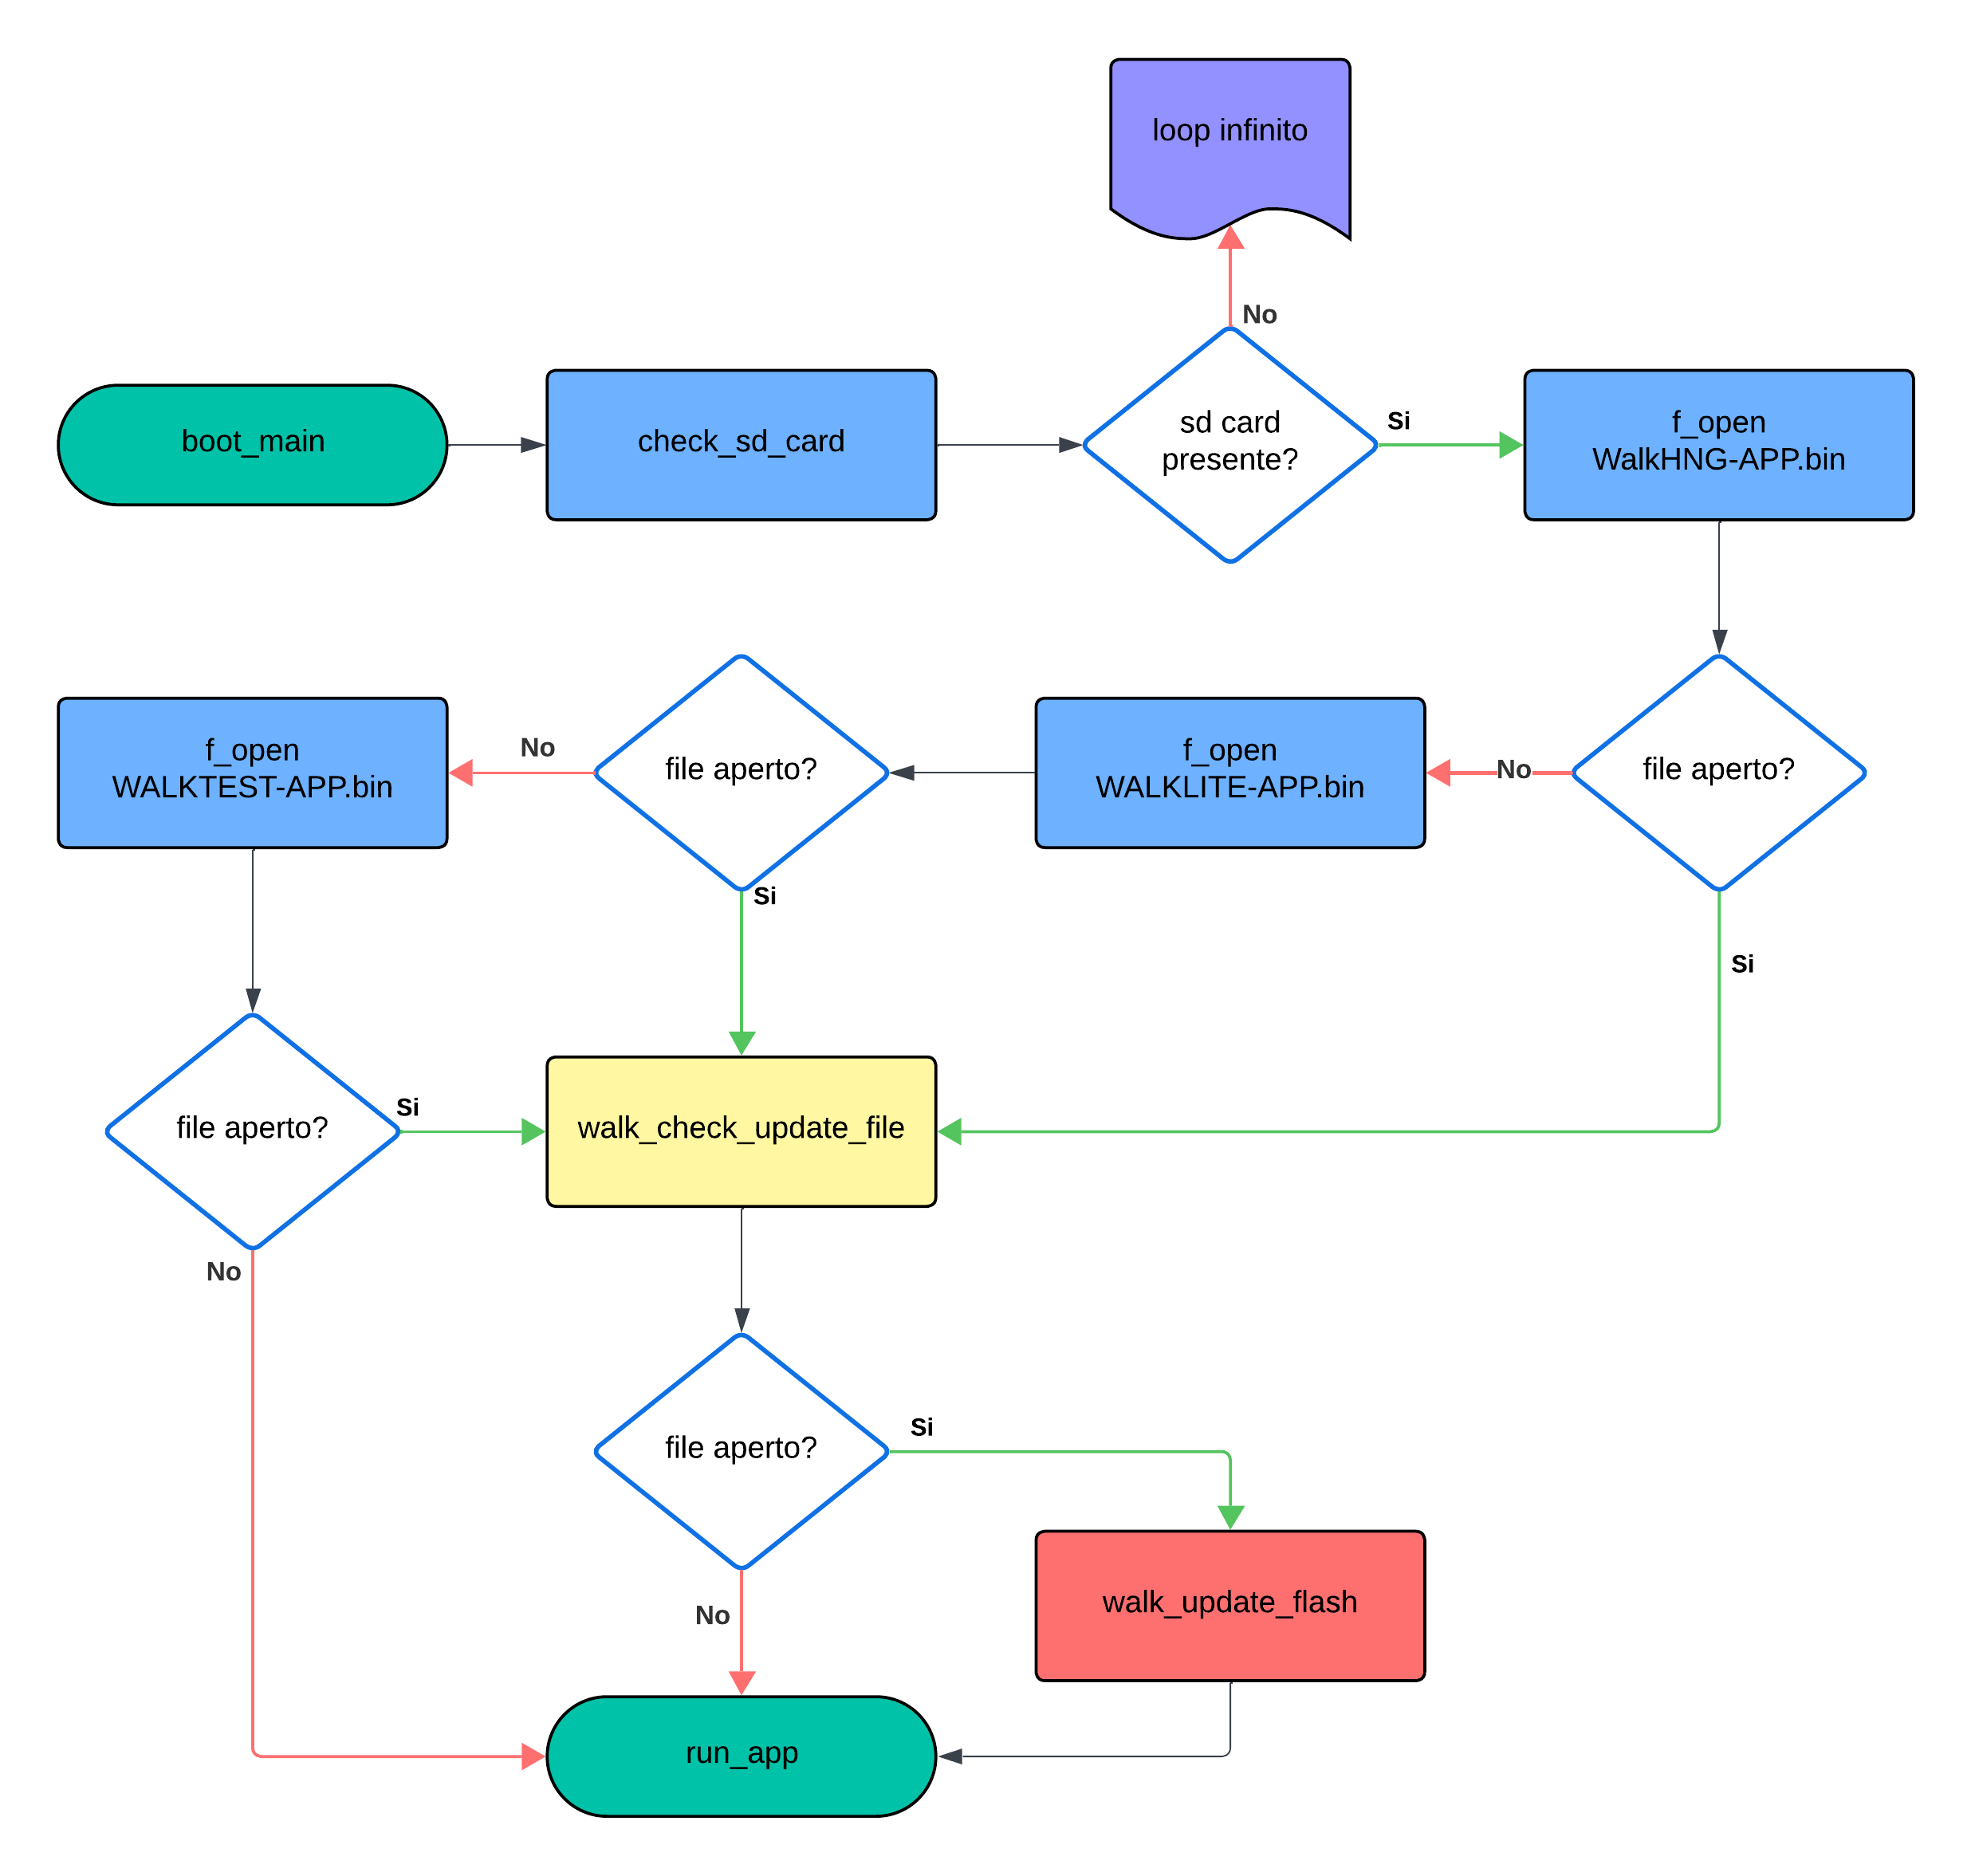
\includegraphics[width=0.8\textwidth]{img/bootloader-flowchart.png}
        \caption{Flowchart semplificato delle funzioni chiave del bootloader del Walk400h.}
        \label{fig:bootloader-flowchart}
        \end{figure}

        \begin{description}
            \item[\texttt{boot\_main}] punto d'ingresso della logica di avvio, 
            responsabile dell'orchestrazione del processo di verifica e 
            aggiornamento del firmware. \\
            \textbf{Criticità}: componente centrale che decide se procedere 
            con l'aggiornamento sulla base dell'esito di alcune verifiche; 
            un errore di logica in questo punto può compromettere 
            l'intero processo di boot.

            \item[\texttt{walk\_check\_update\_file}]
                verifica della validità del file di aggiornamento 
                (\texttt{WALKLITE-APP.bin}) prima che il relativo contenuto venga 
                scritto in memoria Flash. \\
            \textbf{Criticità}: costituisce l'unico punto di controllo tra un 
                file proveniente da un dispositivo di storage removibile e la 
                scrittura in memoria persistente; una validazione insufficiente a 
                questo livello permetterebbe la scrittura di un firmware non 
                verificato.

            \item[\texttt{walk\_update\_flash}]
                scrittura effettiva del nuovo firmware in memoria 
                Flash. \\
                \textbf{Criticità}: operazione privilegiata e irreversibile; un 
                suo utilizzo scorretto (ad esempio raggiungibile bypassando i 
                controlli di \texttt{walk\_check\_update\_file}) comporterebbe la 
                persistenza di codice malevolo sul dispositivo.

        Di particolare interesse è la funzione \texttt{walk\_check\_update\_file}, che costituisce l'unico punto di controllo del file di aggiornamento prima che questo venga considerato valido. Come mostrato in Figura~\ref{fig:walk-check-update-flowchart}, la funzione verifica dapprima l'esistenza del file e che lo spazio disponibile in Flash sia sufficiente per la sua dimensione dichiarata (\texttt{filinfo.size}); in caso contrario, restituisce \texttt{FR\_INT\_ERR}. Superati questi controlli, legge i primi \texttt{0x20} (32) byte del file in un buffer (\texttt{magic}) e ne verifica il contenuto tramite \texttt{mod\_strcmp} e il confronto di quattro byte in coda al buffer (offset \texttt{0x1c}--\texttt{0x1f}): solo se entrambe le condizioni sono soddisfatte il file viene considerato valido (\texttt{FR\_OK}).

        
        
        \begin{figure}[H]
        \centering
        
\includegraphics[width=0.8\textwidth]{tesi/img/walk_check_update_file_flowchart.png}
        \caption{Flowchart semplificato della funzione walk\_check\_update\_file.}
        \label{fig:walk_check_update_file_flowchart}
        \end{figure}
        \end{description}
    
    \section{Meccanismi di monitoraggio implementati}
    \label{subsec:meccanismi_di_monitoraggio}
        Nell'ottica di validare i risultati dell'analisi statica condotta in questa sezione e descritta nel lavoro di Alberici~\cite{alberici26}, e per supportare la successiva esplorazione simbolica del medesimo percorso con gli strumenti di analisi utilizzati, sono stati implementati due meccanismi di osservabilità del comportamento del firmware: il primo consente di monitorare i messaggi stampati via UART, il secondo di rilevare le scritture sulla periferica di memoria Flash. Entrambi i meccanismi sono descritti in seguito.

        \paragraph{Cattura dei messaggi UART}
            Il primo meccanismo ha l'obiettivo di monitorare i messaggi di logging emessi dal firmware via UART durante l'esecuzione simbolica: poiché tali messaggi descrivono in linguaggio naturale le fasi attraversate dal firmware (avvio, verifica della SD Card, validazione del file, ecc.), la loro cattura consente di ricostruire a posteriori quali rami decisionali siano stati attraversati lungo ciascun percorso esplorato, senza dover analizzare manualmente lo stato simbolico a ogni diramazione.

        \paragraph{Monitoraggio della Flash}
            Il secondo meccanismo ha l'obiettivo di rilevare il momento in cui il firmware tenta effettivamente una scrittura nella regione di Flash riservata all'applicazione: individuare questo istante è essenziale per poter osservare, e non solo dedurre indirettamente, se e quando il processo di aggiornamento del firmware giunga a compimento, superando l'intera catena di controlli descritta in precedenza.
\chapter{Metodologia}
        \section{Approccio RetDec + KLEE}
            
            \subsection{Pipeline di decompilazione}
                Per poter applicare KLEE al firmware del Walk400h è stato necessario ottenere una rappresentazione in LLVM IR, formato su cui l'engine di symbolic execution opera nativamente. A tale scopo, il binario raw estratto ed analizzato nel punto 4.2 è stato passato in input a RetDec con i parametri architetturali individuati in fase di reverse engineering (modalitá THUMB, entry point e indirizzo di caricamento), ottenendo come output il bitcode LLVM corrispondente.
    
                Poichè RetDec non riusciva a completare la decompilazione dell'intero file binario del firmware -- la cui dimensione originale è di 1 MB --, sono stati estratti solo i primi 256 KB. Questa strategia è giustificata dal layout standard della memoria flash ARM Cortex-M e verificata tramite l'analisi con Ghidra:
                    \begin{itemize}[noitemsep]
                        \item \textbf{Vector table}: 0x08000000 - 0x080003FF, ~1KB
                        \item \textbf{codice eseguibile}: 0x08000400 - ~0x08028200 (~160KB)
                        \item \textbf{dati statici}: resto del binario
                    \end{itemize}
    
                Lo script per l'estrazione e la decompilazione è riportato di seguito.

                \bashfile{../retdec_klee/retdec_pipeline.sh}

                \subsection{Costruzione del modulo eseguibile}
                
                Il bitcode prodotto da RetDec non è direttamente eseguibile da KLEE: 
                il suo utilizzo ha richiesto la risoluzione di una serie di 
                incompatibilità strutturali, riassunte in 
                Tabella~\ref{tab:klee-module}, individuate in modo incrementale a 
                partire dagli errori restituiti da \texttt{llvm-as} e da KLEE stesso.
                
                \begin{table}[h]
\centering
\small
\begin{tabular}{p{3.2cm} p{4.5cm} p{4.8cm}}
\toprule
\textbf{Problema} & \textbf{Sintomo} & \textbf{Soluzione} \\
\midrule
Variabili globali malformate & 
\texttt{invalid use of function-local name} in fase di assemblaggio & 
Normalizzazione delle dichiarazioni tramite sostituzione testuale mirata \\
\midrule
Entry point mancante & 
\texttt{KLEE: ERROR: Entry function 'main' not found} & 
Creazione di un modulo wrapper con \texttt{main()}, che invoca 
\texttt{boot\_main} con argomenti resi simbolici, linkato al bitcode 
del bootloader \\
\midrule
Conflitti di target/data layout e simboli duplicati & 
Warning di linking e funzioni non risolte & 
Normalizzazione di target triple/datalayout; funzioni originali 
dichiarate a \textit{weak linkage} \\
\midrule
Variabile globale non caricabile & 
\texttt{KLEE: ERROR: Unable to load symbol() while initializing globals} & 
Ridefinizione della variabile da globale esterna a globale 
inizializzata a 0 \\
\bottomrule
\end{tabular}
\caption{Problemi riscontrati nella costruzione del modulo eseguibile e relative soluzioni.}
\label{tab:klee-module}
\end{table}
            \FloatBarrier

            \cfile{../retdec_klee/wrappers/wrapper.c}
            
            \subsection{Stub delle periferiche e simbolizzazione mirata}
                Oltre ai conflitti strutturali descritti in Sezione~5.1.2, l'esecuzione 
                simbolica ha incontrato limitazioni legate all'assenza di un modello 
                per le periferiche hardware e alla gestione delle variabili locali, 
                riassunte in Tabella~\ref{tab:klee-stub}.
                \am{Ti consiglio di mettere le tabelle in file a parte, vedi quella sopra}
                \begin{table}[h]
                \centering
                \small
                \begin{tabular}{p{3.2cm} p{4.5cm} p{4.8cm}}
                \toprule
                \textbf{Problema} & \textbf{Sintomo} & \textbf{Soluzione} \\
                \midrule
                Accessi hardware non modellabili & 
                \texttt{KLEE: ERROR: invalid pointer: klee\_make\_symbolic} su registri 
                MMIO & 
                Sanitizzazione del bitcode: sostituzione dei \texttt{load} da 
                indirizzi hardware e rimozione delle \texttt{store} corrispondenti \\
                \midrule
                Variabile locale passata per riferimento & 
                \texttt{Wrong size given to klee\_make\_symbolic} & 
                Sostituzione, a livello di LLVM IR, del riferimento allo stack con una 
                variabile globale dedicata (buffer \texttt{magic}) \\
                \bottomrule
                \end{tabular}
                \caption{Problemi riscontrati nella simbolizzazione degli input e relative soluzioni.}
                \label{tab:klee-stub}
            \end{table}
            Un vincolo più generale di KLEE, riscontrato nel tentativo di 
            simbolizzare direttamente il buffer di destinazione all'interno dello 
            stub di \texttt{f\_read}, riguarda l'impossibilità di rendere simbolici 
            indirizzi appartenenti allo spazio di memoria del programma stesso 
            (ad esempio un puntatore a una variabile locale sullo stack) tramite 
            una semplice chiamata a \texttt{klee\_make\_symbolic} sul puntatore 
            ricevuto come parametro: il tentativo produceva un arresto immediato 
            dell'esecuzione. Questo vincolo, sommato a quello sulle variabili locali 
            passate per riferimento, ha reso necessaria la strategia di riscrittura 
            manuale del bitcode descritta di seguito.

            Le parti di codice riportate sotto mostrano il confronto tra il codice 
            LLVM IR prima e dopo la riscrittura: il riferimento allo stack 
            (\texttt{\%stack\_var\_-40}), passato come secondo argomento alla 
            chiamata a \texttt{f\_read}, viene sostituito con la variabile globale 
            \texttt{@klee\_magic\_buffer}.
            
\begin{llvmcode}
dec_label_pc_8007e24:
  %15 = call i32 @function_8007e38(i32 9792, i32* nonnull %stack_var_-40, i32 %14, i32* nonnull %stack_var_-76), !insn.addr !6891
  %16 = call i32 @function_8007e76(i32 9792)
  ret i32 2
\end{llvmcode}

\begin{llvmcode}
dec_label_pc_8007c14:
  %114 = call i32 @function_8007e38(i32 9792, ptr nonnull @klee_magic_buffer, i32 32, ptr nonnull %stack_var_-76), !insn.addr !1382
  %115 = call i32 @function_8007874(i32 9792)
  br label %common_ret
\end{llvmcode}
   \FloatBarrier
        
        \section{Approccio Angr}
        \subsection{Configurazione del progetto ed esecuzione Blind}
        Il progetto Angr è stato configurato specificando l'architettura (\texttt{ARMCortexM}), l'indirizzo di caricamento (\texttt{0x08000000}) e l'entry point del bootloader individuato nella \Cref{subsec:firmware_re}, con il bit THUMB abilitato.
        
        \pythonfile{../angr/blind_exploration.py}
        
        Un primo tentativo ha adottato un'esecuzione simbolica ``blind'', priva di un target specifico: l'esplorazione avanza istruzione per istruzione su tutti i percorsi raggiungibili, terminando quando non restano piú stati attivi. Questo approccio si è rivelato inefficiente, poichè l'assenza di un obiettivo non consente di indirizzare l'esplorazione verso le funzioni di interesse.

        \am{Secondo me qui sotto sarebbe buona cosa far vedere dove si ferma}
        Oltre all'inefficienza, l'esecuzione blind si arresta dopo poche istruzioni: l'analisi dello stato mostra che il flusso rimane bloccato all'interno di cicli di attesa legati all'inizializzazione delle periferiche hardware, cicli che in 
        ambiente simbolico non terminano mai poichè i registri hardware non vengono aggiornati da un controllore fisico esterno. Per questo problema sono state valutate due soluzioni:
        \begin{itemize}
            \item Modellazione simbolica delle periferiche: rendere simboliche zone di memoria MMIO, permettendo ad Angr di esplorare tutti i possibili stati dei registri
            \item Stub delle funzioni bloccanti: Sostituzione delle funzioni che dipendono dai cicli di attesa hardware 
con procedure che restituiscono immediatamente un valore fisso
        \end{itemize}

        \subsection{Intercettazione UART}
        Nell'ambito dell'esecuzione blind è stata inoltre condotta la cattura dei messaggi di debug a livello di registro, allo scopo di identificare quale periferica seriale fosse effettivamente utilizzata dal firmware. A partire dagli indirizzi delle periferiche USART/UART riportati nel datasheet del microcontrollore, sono stati impostati dei breakpoint di memoria sui rispettivi registri \textbf{TDR} (Transmit Data Register, ovvero a un offset di +0x28 rispetto all'indirizzo base di ciascuna periferica). 

        Come anticipato nella sezione 5.2.1, l'esecuzione simbolica ``blind'' non riesce a superare nemmeno l'inizializzazione delle periferiche hardware, rimanendo bloccata in dei cicli. È stato quindi necessario applicare alle funzioni bloccanti degli stub per permettere l'avanzamento dell'esecuzione. Questo è stato possibile tramite l'analisi del decompilato su Ghidra, dimostrando come un approccio totalmente ``blind'' sia impraticabile.
        \newline
        Il codice sottostante è quello relativo alla cattura UART; sono 
        riportate solamente le parti aggiuntive rispetto al codice base 
        dell'esecuzione blind già mostrato in Sezione 5.2.1.
        \inputminted[
            frame=single,
            linenos,
            breaklines,
            bgcolor=gray!10,
            firstline=1,
            lastline=30,
            firstnumber=1
        ]{python}{../angr/USART.py}
    
        \inputminted[
            frame=single,
            linenos,
            breaklines,
            bgcolor=gray!10,
            firstline=46,
            lastline=59,
            firstnumber=46
        ]{python}{../angr/USART.py}

    Output:

    \begin{minted}[frame=single, breaklines, bgcolor=gray!10, fontsize=\footnotesize]{text}
        simgr: <SimulationManager with 1 active>, active: [<SimState @ 0x80054e1>], errored: [], deadneded: [] 0x40004828 -> W
        simgr: <SimulationManager with 1 active>, active: [<SimState @ 0x80054e1>], errored: [], deadneded: [] 0x40004828 -> a
        simgr: <SimulationManager with 1 active>, active: [<SimState @ 0x80054e1>], errored: [], deadneded: [] 0x40004828 -> l
        [...]
        simgr: <SimulationManager with 1 active>, active: [<SimState @ 0x80054e1>], errored: [], deadneded: [] 0x40004828 -> 0
        simgr: <SimulationManager with 1 active>, active: [<SimState @ 0x80054e1>], errored: [], deadneded: [] 0x40004828 -> 6
    \end{minted}

    \am{Ho visto che c 'è la sezione 5.2.3 per gli stub. Mettila prima di questa e menziona il problema (quindi funzioni che si bloccano, degli stub, che per capire dove metterli hai bisogno di una qualche analisi altrimenti devi mettere tutta la memoria simbolica, ecc) una sola volta così evitiamo di ripeterlo}
    L'intercettazione a livello di registro si è rivelata funzionante - il breakpoint sui registri TDR ha permesso di identificare USART3 come periferica di logging - ma computazionalmente onerosa: il tempo di esecuzione cresce rapidamente all'aumentare del numero di stati simbolici attivi rendendolo poco praticabile su esplorazioni più estese. A questo scopo, nelle analisi successive, si è preferito adottare la cattura dei messaggi di debug con un meccanismo basato su hooking della funzione \texttt{printf}, meno oneroso in termini prestazionali.

    Oltre all'hooking, è stato aggiunto un meccanismo di logging dei messaggi di debug: questo meccanismo utilizza la funzionalitá dei \texttt{plugin} di Angr. I plugin sono delle estensioni dello stato che permettono di memorizzare dati custom durante l'esecuzione simbolica e vengono automaticamente duplicati quando si forka lo stato, garantendo che ogni branch mantenga la propria copia indipendente dei messaggi.
    È possibile registrare un nuovo plugin attraverso il comando:
    \begin{minted}[frame=single, breaklines, bgcolor=gray!10, fontsize=\footnotesize]{python}
        state.register_plugin('printf_log', PrintfLogger())
    \end{minted}

    La classe \texttt{HookPrintf} si occupa dell'hooking della funzione 
    \texttt{printf} e svolge i seguenti compiti:
    
    \begin{itemize}[noitemsep]
        \item intercetta le chiamate a \texttt{printf} durante l'esecuzione simbolica;
        \item estrae la format string e i primi tre argomenti, letti dai 
        registri \texttt{r1}, \texttt{r2} e \texttt{r3} secondo la calling 
        convention ARM;
        \item gestisce i format specifier più comuni (\texttt{\%s}, 
        \texttt{\%d}, \texttt{\%u}, \texttt{\%x});
        \item nel caso di \texttt{\%x}, converte il valore in carattere 
        ASCII se stampabile, altrimenti lo riporta in formato esadecimale;
        \item salva il messaggio formattato nel plugin \texttt{PrintfLogger}.
    \end{itemize}

    \subsection{Stub per l'esplorazione}
    Per ridurre il numero di stati simbolici da esplorare e guidare l'esecuzione verso il flusso di aggiornamento del firmware, sono stati introdotti stub di due tipologie:
    \begin{itemize}
        \item \textbf{Stub di funzioni rilevanti o che restituiscono valore fisso}: sostituiscono con un'istruzione vuota (\textbf{DoNothing}) le funzioni che non influenzano il flusso di aggiornamento del firmware, ma la cui esecuzione introdurrebbe stati superflui, come routine di inizializzazione.
        \item \textbf{Stub che ritornano un valore fisso}: sostituiscono funzioni il cui esito è necessario per proseguire lungo il percorso di interesse, forzando il valore di ritorno anzichè eseguire la logica reale - ad esempio \texttt{check\_sd\_card}, per garantire che la scheda SD risulti 
        sempre presente o le funzioni HAL di gestione della Flash 
        (\texttt{HAL\_FLASH\_Unlock}, \texttt{HAL\_FLASHEx\_Erase}), le cui 
        operazioni sulla memoria fisica non sono riproducibili in ambiente 
        simbolico.
    \end{itemize}
    
    
    \subsection{Modellazione di FatFS}
    \am{Forse metterei giusto una frase per dire che adesso vogliamo modellare la parte di aggiornamento quindi ci servono le funzioni per leggere il FS}
        Le funzioni di libreria FATFS operano su strutture dati con un layout preciso (\texttt{FIL}, \texttt{FILINFO}), i cui campi vengono letti e scritti dal firmware in punti diversi del flusso di validazione. Per poter riferire questi campi per nome anzichè calcolarne manualmente l'offset in memoria, le definizioni di questo tipo di FatFS sono state registrate in Angr tramite \texttt{Angr.types.register\_types}, fornendo un equivalente dei \textbf{typedef} originali.

        \inputminted[
            frame=single,
            linenos,
            breaklines,
            bgcolor=gray!10,
            firstline=4,
            lastline=45,
            firstnumber=4
        ]{python}{../angr/moduli/boot_hook.py}

        Su questa base sono stati poi implementati gli hook \texttt{HookFRead} e \texttt{HookFStat}, che costituiscono l'esecuzione reale delle rispettive funzioni FatFS.

        \begin{minted}[frame=single, breaklines, bgcolor=gray!10, fontsize=\footnotesize]{python}
    class HookFRead(Angr.SimProcedure):
        def run(self, fil, buf, count, read_ptr):
            ret_addr = hex(self.state.callstack.ret_addr)
            position = self.state.solver.eval(self.state.mem[fil].FIL.fptr.resolved)
            real_count = self.state.solver.eval(count)
                    
            fill_info_obj = claripy.BVS(f'f_read_{hex(position)}_{hex(real_count)}_{ret_addr}', real_count * self.state.arch.bits)
            self.state.memory.store(buf, fill_info_obj, real_count, disable_actions=True, inspect=False)
            self.state.memory.store(read_ptr, real_count, 4, disable_actions=True, inspect=False)
            
            self.state.mem[fil].FIL.fptr = position + real_count
                        
            return 0 
            
    class HookFStat(Angr.SimProcedure):
        def run(self, file_path, fill_info):
            size = self.state.mem.FILINFO._type.size // 8
            ret_addr = hex(self.state.callstack.ret_addr)
            fill_info_obj = claripy.BVS(f'f_stat_{file_path}_{ret_addr}', size * self.state.arch.bits)
            self.state.memory.store(fill_info, fill_info_obj, size, disable_actions=True, inspect=False)            
            return 0
        \end{minted}        

        \begin{itemize}[noitemsep]
            \item \texttt{HookFRead} non modella l'accesso reale al filesystem 
            sulla SD Card, ma scrive nel buffer di destinazione (\texttt{buf}) 
            una variabile simbolica di dimensione pari alla quantità richiesta 
            (\texttt{count}), aggiornando contestualmente il campo \texttt{fptr} 
            della struttura \texttt{FIL} e il numero di byte letti 
            (\texttt{read\_ptr}). Il nome della variabile simbolica contiene 
            posizione, quantità richiesta e indirizzo di ritorno della chiamata, 
            garantendo che letture diverse generino variabili indipendenti 
            anzichè condividere lo stesso valore simbolico.
            \item \texttt{HookFStat} rende simbolica l'intera struttura di \texttt{FILINFO} restituita al chiamante
        \end{itemize}

        Questo approccio permette al solver di determinare automaticamente quali valori concreti di questi campi soddisfano i vincoli imposti dalla logica di validazione del firmware.
        
    \subsection{Esplorazione percorsi}
        
        Per rendere l'esplorazione mirata anzichè esaustiva, è stata adottata 
        la funzione \texttt{simgr.explore()} di Angr, configurabile tramite tre 
        parametri principali:

        \begin{itemize}[noitemsep]
            \item un \textbf{target}: l'indirizzo che l'esecuzione deve 
            raggiungere per considerarsi conclusa con successo;
            \item uno o più indirizzi da \textbf{evitare}, che vengono scartati 
            non appena raggiunti;
            \item un numero massimo di step, oltre il quale l'esplorazione si 
            interrompe anche in assenza di stati che soddisfino la condizione 
            di target.
        \end{itemize}
        
        Come target è stato scelto l'indirizzo di \texttt{walk\_update\_flash}, 
        funzione responsabile della scrittura del firmware in memoria Flash, 
        mentre come indirizzo da evitare è stato specificato \texttt{run\_app}, 
        corrispondente all'avvio dell'applicativo principale: questo evita che 
        l'esecuzione prosegua oltre il bootloader una volta completato il flusso 
        di aggiornamento.
        
        \inputminted[
            frame=single,
            linenos,
            breaklines,
            bgcolor=gray!10,
            firstline=94,
            lastline=101,
            firstnumber=94
        ]{python}{../angr/boot_main_exploration.py}
        
        L'esplorazione condivide con l'esecuzione blind gli stub per le funzioni 
        di inizializzazione e utilizza l'hook di \texttt{printf} descritto in 
        Sezione~5.2.2. A questi si aggiungono gli stub mirati a guidare il 
        flusso di esecuzione verso \texttt{walk\_update\_flash}, insieme agli 
        hook per la modellazione di FatFS descritti in Sezione~5.2.4. In questo 
        modo, se l'esplorazione raggiunge il target, il solver di Angr può 
        essere interrogato per determinare quali valori delle variabili rese 
        simboliche soddisfano i vincoli imposti dalla funzione 
        \texttt{walk\_check\_update\_file}.

    \subsection{Breakpoint in memoria}
        Il secondo approccio target-oriented adottato è basato su un breakpoint in memoria e condivide gran parte della struttura con il metodo precentente: la configurazione del progetto, gli stub e la modellazione di FatFS restano invariati. La differenza risiede nel criterio con cui l'esplorazione viene considerata conclusa.

        Mentre l'esplorazione termina quando si raggiunge un determinato indirizzo, l'approccio a breakpoint termina quando si verifica quando viene rilevata una scrittura nella regione di Flash riservata all'applicazione. A tale scopo viene registrato un breakpoint di inspection sull'evento di scrittura in memoria, filtrato sull'indirizzo di tale regione (\texttt{FLASH\_BASE}, \texttt{0x0800e000}); alla prima scrittura rilevata, il relativo handler imposta un flah nello stato corrente, che diventa la condizione di terminazione passata a \texttt{simgr.explore()}.

        \inputminted[
            frame=single,
            linenos,
            breaklines,
            bgcolor=gray!10,
            firstline=97,
            lastline=106,
            firstnumber=97
        ]{python}{../angr/boot_main_memory_hooks.py}
    \chapter{Risultati}
        \section{RetDec + Klee}
            L'esecuzione simbolica della pipeline RetDec + Klee non ha prodotto risultati significativi per quanti riguarda l'analisi, mettendo in luce le difficoltá di questi strumenti per analizzare un firmware embedded reale.

            \subsection{Esiti dell'esecuzione}
            L'esecuzione con KLEE è terminata dopo 277 istruzioni, con un solo percorso esplorato in modo parziale e nessun percorso completato. La terminazione è avvenuta in corrispondenza di un accesso a puntatore non valido (\texttt{null page access}), senza che l'esecuzione raggiungesse la logica di validazione del \textit{magic number} all'interno di \texttt{walk\_check\_update\_file}. Nonostante ció l'output mostra che la pipiline è comunque riuscita ad avanzare fino all'ingresso di \texttt{walk\_check\_update\_file}, superando le fasi di inizializzazione grazie agli stub creati.

            \subsection{Decompilazione incompleta}
            L'analisi della causa del mancato raggiungimento della logica di controllo del \textit{magic number} ha evidenziato il problema principale di questo approccio: il codice prodotto da Retdec non è funzionalmente equivalente al binario originale. Confrontando il decompilato (nelle sue forme pseudo-C e LLVM IR) con il disassemblato Ghidra emergono infatti delle omissioni significative.

            In particolare, all'interno di \texttt{walk\_check\_update\_file} manca completamente il ramo di validazione \textit{magic number}. La mancanza di questo questo ramo impedisce a KLEE di esplorare i percorsi che attraversano la validazione del file di aggiornamento, ossia proprio la logica di interesse per l'analisi.

            Non è possibile escludere che l'output di RetDec presenti ulteriori omissioni analoghe per altre porzioni di codice.

            Decompilato Ghidra (il ramo di validazione, con 
            \texttt{mod\_strcmp}, \texttt{strcpy}, ...)
            
            \begin{minted}[frame=single, breaklines, bgcolor=gray!10, fontsize=\footnotesize]{c}
if (res == FR_OK) {
    f_close(&file_struct);
    magic[7] = '\0';
    cmp_res = mod_strcmp("WalkHNG", magic);
    if ((((cmp_res == 0) && (magic[0x1c] == -0x41)) && (magic[0x1d] == -3)) &&
        ((magic[0x1e] == -0x2f && (magic[0x1f] == '\x1c')))) {
        magic[0xf] = '\0';
        magic[0x1b] = '\0';
        strcpy(&global_magic, magic + 8);
        strcat(&global_magic, " v");
        strcat(&global_magic, magic + 0x10);
        putc_state = '\0';
        printf("--> Load File: %s\r", filinfo.fname);
        printf("--> size: %d bytes\r", filinfo.fsize);
        printf("--> Code: %s\r", &global_magic);
        return FR_OK;
    }
}
\end{minted}

Decompilato RetDec (la stessa funzione: dopo \texttt{f\_read} salta direttamente a \texttt{f\_close} e \textit{return 2}, il ramo di validazione non c'è):
\begin{minted}[frame=single, breaklines, bgcolor=gray!10, fontsize=\footnotesize]{c}
int32_t walk_check_update_file(void) {
    // 0x8007be4
    int32_t v1; // bp-72, 0x8007be4
    memset(&v1, 0, 32);
    int32_t v2 = 0; // bp-76, 0x8007bf4
    if (f_stat(*(int32_t *)0x20002400, &v1) != 0) {
        // 0x8007cb8
        return 2;
    }
    uint16_t v3 = *(int16_t *)0x1fff75e0; // 0x8007c06
    if (v3 == -1) {
        __asm_it();
    } else {
        __asm_itttt();
    }
    if ((v3 == -1 ? 0xf2000 : (1024 * (int32_t)v3 & 0x3ffc00) - 0xe000) < v1) {
        // 0x8007cb8
        return 3;
    }
    // 0x8007c24
    int32_t v4; // bp-40, 0x8007be4
    f_read(0x2640, &v4, 32, &v2);
    f_close(0x2640);
    return 2;
}
\end{minted}
        \section{Angr}
        \subsection{Esplorazione dei percorsi}
        
        L'esplorazione dei percorsi ha raggiunto con successo la funzione 
        target \texttt{walk\_update\_flash}: il \textit{simulation manager} 
        riporta uno stato in \texttt{found}, a fronte di 95 stati ancora attivi 
        e 12 scartati perchè diretti verso l'indirizzo da evitare.
        
        \paragraph{Struttura del magic number}
        
        Interrogando il solver sui vincoli accumulati lungo il percorso, è 
        possibile ricostruire la sequenza di byte che il file di aggiornamento 
        deve contenere per superare la validazione. I 14 vincoli individuati si 
        traducono nella seguente struttura dell'header:
        
        \begin{table}[H]
        \centering
        \small
        \begin{tabular}{c c c}
        \toprule
        \textbf{Offset (byte)} & \textbf{Valore} & \textbf{Interpretazione} \\
        \midrule
        0--6   & \texttt{57 61 6c 6b 48 4e 47} & \texttt{"WalkHNG"} \\
        \midrule
        8, 16  & \texttt{00} & padding \\
        \midrule
        28--31 & \texttt{bf fd d1 1c} & fine magic \\
        \bottomrule
        \end{tabular}
        \caption{Decodifica dei vincoli sul buffer letto da \texttt{f\_read}.}
        \label{tab:magic-constraints}
        \end{table}
        \FloatBarrier
        
        Si osserva, dal disassemblato Ghidra, che solo i primi 7 byte (il magic 
        \texttt{"WalkHNG"}) e gli ultimi 4 byte (\texttt{bf fd d1 1c}) sono 
        effettivamente vincolanti ai fini della validazione; i byte del padding 
        possono assumere un valore qualsiasi eccetto per il primo e l'ultimo che sono vincolati.
        
        Il primo vincolo coinvolge invece la variabile simbolica creata in 
        \texttt{HookFStat}, corrispondente all'intera struttura 
        \texttt{FILINFO}: la porzione selezionata (\texttt{[703:672]}) isola il 
        campo \texttt{fsize}, mentre \texttt{Reverse(...)} corregge l'ordine 
        dei byte per l'endianness little-endian del microcontrollore. Il 
        vincolo lega \texttt{filinfo.fsize} al valore di \texttt{available} 
        calcolato dal firmware: per lo stato trovato, il solver ammette valori 
        di \texttt{filinfo.fsize} fino a \texttt{0xffff2000} ($\sim$4\,GB), 
        coerentemente con la vulnerabilità di integer underflow discussa in 
        Sezione~6.2.3.

\begin{minted}[frame=single, breaklines, bgcolor=gray!10, fontsize=\footnotesize]{text}
Total constraints: 14

  [ 1] <Bool 0xffff2000 >= Reverse(f_stat_<BV32 0x800bcd2>_0x8007c01_965_704[703:672])>
  [ 2] <Bool f_read_0x0_0x20_0x8007c31_966_1024[1023:1016] == 87>
  [ 3] <Bool f_read_0x0_0x20_0x8007c31_966_1024[1015:1008] == 97>
  [ 4] <Bool f_read_0x0_0x20_0x8007c31_966_1024[1007:1000] == 108>
  [ 5] <Bool f_read_0x0_0x20_0x8007c31_966_1024[999:992] == 107>
  [ 6] <Bool f_read_0x0_0x20_0x8007c31_966_1024[991:984] == 72>
  [ 7] <Bool f_read_0x0_0x20_0x8007c31_966_1024[983:976] == 78>
  [ 8] <Bool f_read_0x0_0x20_0x8007c31_966_1024[975:968] == 71>
  [ 9] <Bool f_read_0x0_0x20_0x8007c31_966_1024[799:792] == 191>
  [10] <Bool f_read_0x0_0x20_0x8007c31_966_1024[791:784] == 253>
  [11] <Bool f_read_0x0_0x20_0x8007c31_966_1024[783:776] == 209>
  [12] <Bool f_read_0x0_0x20_0x8007c31_966_1024[775:768] == 28>
  [13] <Bool f_read_0x0_0x20_0x8007c31_966_1024[959:952] == 0>
  [14] <Bool f_read_0x0_0x20_0x8007c31_966_1024[895:888] == 0>
\end{minted}

\paragraph{Call Stack}

\begin{minted}[frame=single, breaklines, bgcolor=gray!10, fontsize=\footnotesize]{text}
0 | boot_main -> walk_update_flash, returning to boot_main
1 | 0x0 -> 0x0, returning to 0x0
\end{minted}

        \paragraph{Execution Path}
        
        A differenza dell'approccio RetDec + KLEE (Sezione~6.1), compare qui il 
        branch di validazione del magic number, con le chiamate a 
        \texttt{mod\_strcmp}, \texttt{strcpy} e \texttt{strcat}.

\begin{minted}[frame=single, breaklines, bgcolor=gray!10, fontsize=\scriptsize]{text}
boot_reset_handler
+-- boot_main
    +-- HAL_Init
    +-- walk_uart_setup
    +-- check_sd_card
    +-- f_open
    +-- walk_check_update_file
    |   +-- f_stat
    |   +-- f_read
    |   +-- mod_strcmp
    |   +-- strcpy
    |   +-- strcat
    |   [...]
    +-- walk_preparing_flash
    |   +-- HAL_FLASH_Unlock
    +-- walk_do_flash_programming
    +-- walk_update_flash
Total jumps (jumpkinds): 2794
\end{minted}

        \paragraph{Printf Logs}
        
        A chiusura dell'esecuzione vengono riportati i log di debug, che 
        raccontano in modo più immediato il percorso seguito.

\begin{minted}[frame=single, breaklines, bgcolor=gray!10, fontsize=\footnotesize]{text}
[ 1] **** WalkHNG Boot v 1.06 ****
[ 2] --> Debug usart ready...
[ 3] --> Start Buzzer driver
[ 4] --> Start TFT driver
[ 5] Check file WalkHNG-APP.bin
[ 6] Found upload file WalkHNG-APP.bin
[ 7] -> Load File:
[ 8] -> size: 0 bytes
[ 9] -> Code:  v
[10] --> Update ready, Left skip, right go update
\end{minted}

    \subsection{Breakpoint in memoria}
    Anche l'approccio a breakpoint in memoria ha raggiunto con successo il proprio criterio di terminazione: il \textit{simulation manager} riporta uno stato in \texttt{found}, a fronte di 191 stati ancora attivi, nessuno stato scartato e nessuno stato in errore.

    Rispetto all'esplorazione dei percorsi, sia il numero di stati complessivi sia il numero di salti risultano superiori riflettendo la maggior profonditá raggiunta dall'esecuzione: mentre l'esplorazione si ferma a \texttt{walk\_update\_flash}, il breakpoint in memoria arriva fin dentro a \texttt{HAL\_FLASH\_Program}, la funzione che esegue effettivamente la scrittura su Flash.

    \paragraph{Scrittura in Flash rilevata}

        Il breakpoint sul registro \texttt{mem\_write} è scattato in due 
        occasioni, corrispondenti a due scritture consecutive di una word 
        (4 byte) a partire dall'indirizzo \texttt{0x0800e000}, corrispondente 
        all'inizio della regione Flash applicativa:
\begin{minted}[frame=single, breaklines, bgcolor=gray!10, fontsize=\footnotesize]{text}
[FLASH] Scrittura a 0x800e000, Valore: <BV32 f_read_0x20_0x2000_0x8007d25_1060_262144[262119:262112] .. 
    f_read_0x20_0x2000_0x8007d25_1060_262144[262127:262120] .. 
    f_read_0x20_0x2000_0x8007d25_1060_262144[262135:262128] .. 
    f_read_0x20_0x2000_0x8007d25_1060_262144[262143:262136]>
[FLASH] Scrittura a 0x800e000, Valore: <BV32 f_read_0x20_0x2000_0x8007d25_1062_262144[262119:262112] .. 
    f_read_0x20_0x2000_0x8007d25_1062_262144[262127:262120] .. 
    f_read_0x20_0x2000_0x8007d25_1062_262144[262135:262128] .. 
    f_read_0x20_0x2000_0x8007d25_1062_262144[262143:262136]>
\end{minted}

        \paragraph{Constraints}
        
        Rispetto all'esplorazione dei percorsi (Tabella~\ref{tab:magic-constraints}), 
        il numero di vincoli è salito da 14 a 17: ai 14 vincoli già discussi, 
        che fissano il contenuto del \textit{magic number}, si aggiungono tre vincoli 
        derivanti da una seconda invocazione di \texttt{f\_stat} (indirizzo di 
        ritorno \texttt{0x8007e01}), effettuata da \texttt{walk\_program\_flash} 
        prima della scrittura effettiva. Questi vincoli restringono 
        ulteriormente il valore di \texttt{filinfo.fsize} rispetto al primo 
        controllo.

\begin{minted}[frame=single, breaklines, bgcolor=gray!10, fontsize=\footnotesize]{text}
<Bool LShR(Reverse(f_stat_<BV32 0x800bcd2>_0x8007e01_967_704[703:672]), 0xd) != 0x0>
<Bool 0xffff2000 > Reverse(f_stat_<BV32 0x800bcd2>_0x8007e01_967_704[703:672])>
<Bool 0x0 <=s (0xa7 + (0 .. 0x80 / (0x0 .. f_stat_<BV32 0x800bcd2>_0x8007e01_967_704[679:672] .. 
    f_stat_<BV32 0x800bcd2>_0x8007e01_967_704[687:680] .. 
    f_stat_<BV32 0x800bcd2>_0x8007e01_967_704[695:693])[7:0]) .. 0x0) >> 0x10>
\end{minted}

\paragraph{Call Stack}

\begin{minted}[frame=single, breaklines, bgcolor=gray!10, fontsize=\footnotesize]{text}
0 | walk_do_flash_programming -> HAL_FLASH_Program, returning to walk_do_flash_programming
1 | walk_program_flash -> walk_do_flash_programming, returning to walk_program_flash
2 | walk_update_flash -> walk_program_flash, returning to walk_update_flash
3 | boot_main -> walk_update_flash, returning to boot_main
4 | 0x0 -> 0x0, returning to 0x0
\end{minted}
A differenza dell'esplorazione dei percorsi, che si ferma all'ingresso 
di \texttt{walk\_update\_flash} con uno stack di profondità 2, qui lo 
stack raggiunge una profondità di 5: l'esecuzione prosegue realmente 
all'interno del flusso di programmazione della Flash, fino a 
\texttt{HAL\_FLASH\_Program}.

\paragraph{Execution Path}

\begin{minted}[frame=single, breaklines, bgcolor=gray!10, fontsize=\scriptsize]{text}
boot_reset_handler
+-- boot_main
    +-- check_sd_card
    +-- f_open
    +-- walk_check_update_file
    |   +-- f_stat
    |   +-- f_read
    |   +-- mod_strcmp
    |   +-- strcpy
    |   +-- strcat
    |   [...]
    +-- walk_preparing_flash
    +-- walk_do_flash_programming
    +-- walk_update_flash
        +-- f_stat
        +-- walk_start_flash_erase
        +-- walk_program_flash
            +-- f_read
            +-- printf  [...]  (33 chiamate)
            +-- walk_do_flash_programming
                +-- HAL_FLASH_Unlock
                +-- HAL_FLASH_Program
                    +-- FLASH_WaitForLastOperation
Total jumps (jumpkinds): 2938
\end{minted}

\begin{minted}[frame=single, breaklines, bgcolor=gray!10, fontsize=\footnotesize]{text}
[ 0] **** WalkHNG Boot v 1.06 ****
[...]
[ 4] Check file WalkHNG-APP.bin
[ 5] Found upload file WalkHNG-APP.bin
[...]
[10] >0x800e000-
[...]  (33 byte, tutti 0x0)
[43] >2097152
\end{minted}

        Le voci dalla [10] alla [43] corrispondono al log emesso da 
        \texttt{walk\_program\_flash} durante la scrittura: l'indirizzo di 
        destinazione, seguito dai byte scritti (qui simbolicamente concretizzati 
        a \texttt{0x0}) e infine dalla dimensione complessiva del file, pari a 
        \texttt{2097152} byte (2\,MB) — un valore che, seppur diverso da quello 
        osservato nell'esplorazione dei percorsi, conferma ulteriormente 
        l'assenza di un limite realistico sulla dimensione ammessa per il file 
        di aggiornamento (Sezione~6.2.3).

    \subsection{La vulnerabilità dell'integer underflow}
        I vincoli osservati sia nell'esplorazione dei percorsi (Sezione~6.2.1) sia nel breakpoint in memoria (Sezione~6.2.2) hanno mostrato che il limite superiore ammesso per \texttt{filinfo.fsize} è nell'ordine dei \texttt{0xffff2000} byte, un valore ($\sim$4\,GB) del tutto incompatibile con la reale capacità della memoria Flash del dispositivo (dell'ordine del MB).

    \paragraph{Il meccanismo}

        Il controllo sulla dimensione del file di aggiornamento, all'interno 
        di \texttt{walk\_check\_update\_file}, si basa sulla variabile 
        \texttt{available}, calcolata a partire dal registro 
        \texttt{\_flash\_size\_data\_register}:

\begin{minted}[frame=single, breaklines, bgcolor=gray!10, fontsize=\footnotesize]{c}
if (_flash_size_data_register == 0xffff) {
    available = (uint32_t)&DAT_000f2000;
} else {
    available = (_flash_size_data_register & 0xfff) * 0x400 - 0xe000;
}
if (available < filinfo.fsize) {
    return FR_NOT_READY;
}
\end{minted}

        Il firmware non convalida il valore di 
        \texttt{\_flash\_size\_data\_register} prima di utilizzarlo nel 
        calcolo. Se tale registro risulta pari a \texttt{0}, l'espressione 
        \texttt{(0 \& 0xfff) * 0x400 - 0xe000} produce un valore negativo 
        (\texttt{-0xe000}); poichè \texttt{available} è dichiarata come 
        \texttt{uint32\_t}, il risultato va incontro a un \textit{integer 
        underflow}, avvolgendosi (\textit{wrap-around}) al valore 
        \texttt{0xffff2000} — un limite superiore di fatto inesistente per la 
        dimensione del file accettato.
        
        \paragraph{Verifica sperimentale}
        
        La vulnerabilità è stata confermata osservando, tramite Angr, come il 
        range di valori ammessi per \texttt{filinfo.fsize} cambi al variare del 
        valore inizializzato in \texttt{\_flash\_size\_data\_register}:
        
        \begin{table}[H]
        \centering
        \small
        \begin{tabular}{c c c}
        \toprule
        \textbf{\texttt{\_flash\_size\_data\_register}} & \textbf{available (atteso)} & \textbf{\texttt{filinfo.fsize} massimo ammesso} \\
        \midrule
        \texttt{0x0000} (non inizializzato) & underflow & \texttt{0xffff2000} ($\sim$4\,GB) \\
        \midrule
        \texttt{0x0400} (1024\,KB reali) & $\sim$968\,KiB & \texttt{991231} byte ($\sim$968\,KiB) \\
        \bottomrule
        \end{tabular}
        \caption{Limite superiore di \texttt{filinfo.fsize} ammesso dal solver, in funzione del valore di \texttt{\_flash\_size\_data\_register}.}
        \label{tab:underflow}
        \end{table}
        \FloatBarrier

        Di seguito è riportato il vincolo che varia nell'esecuzione con \textit{breakpoint in memoria}, impostando \texttt{\_flash\_size\_data\_register = 0x0400}:

\begin{minted}[frame=single, breaklines, bgcolor=gray!10, fontsize=\footnotesize]{c}
  <Bool 0xf2000 > Reverse(f_stat_<BV32 0x800bcd2>_0x8007e01_967_704[703:672])>
\end{minted}
        
        Con il registro correttamente inizializzato a un valore rappresentativo 
        della memoria Flash reale (\texttt{0x0400}), il limite risultante è 
        coerente con lo spazio fisicamente disponibile. Con il registro a 
        \texttt{0} — condizione osservata quando Angr inizializza a zero i 
        registri hardware non vincolati, ma potenzialmente riproducibile anche 
        sul dispositivo reale in assenza di un'inizializzazione esplicita, o 
        tramite manipolazione diretta — il controllo sulla dimensione del file 
        risulta di fatto privo di effetto.

    \section{Vulnerabilità identificate}
    
        Sulla base dei risultati presentati nelle sezioni precedenti, è 
        possibile riassumere le vulnerabilità individuate nel meccanismo di 
        aggiornamento del firmware del Walk400h. Questa sezione si limita a 
        elencarle in modo puntuale.
        \paragraph{Validazione dell'header insufficiente}
            Il firmware accetta come valido qualsiasi file di aggiornamento il cui 
            contenuto inizi con la sequenza di byte determinata in 
            Sezione~6.2 (Tabella~\ref{tab:magic-constraints}):
            
            \begin{itemize}[noitemsep]
                \item magic header: \texttt{"WalkHNG\textbackslash 0"} (7 byte, offset 0--6);
                \item corpo: 20 byte, di cui solo due (offset 8 e 16) risultano 
                effettivamente vincolati dal controllo, entrambi a valore \texttt{0x00};
                \item sequenza di terminazione: \texttt{bf fd d1 1c} (4 byte, offset 28--31).
            \end{itemize}
            
            Nessun altro byte del file, oltre a questi 11, concorre alla decisione 
            di accettare o rifiutare l'aggiornamento.
        
        \paragraph{Assenza di protezione crittografica}
            Il meccanismo di validazione osservato non prevede alcuna forma di 
            verifica dell'autenticità o dell'integrità del file, in particolare:
            
            \begin{itemize}[noitemsep]
                \item non è presente una firma digitale, che consentirebbe di 
                verificare che il file provenga da una fonte autorizzata;
                \item non è presente un meccanismo di checksum o hash, che 
                consentirebbe di rilevare corruzioni o modifiche del file.
            \end{itemize}
        
        \paragraph{Controllo limitato sul nome del file}
            Il controllo sul nome del file di aggiornamento, osservato nell'analisi 
            del bootloader (Sezione~4.3), si limita alla corrispondenza esatta con 
            la stringa \texttt{WalkHNG-APP.bin}, senza ulteriori verifiche sul 
            percorso o sull'origine del file.
        
        \paragraph{Assenza di validazione su \texttt{\_flash\_size\_data\_register}}
        
        Come dimostrato in Sezione~6.2.3, il valore del registro 
        \texttt{\_flash\_size\_data\_register}, utilizzato per calcolare lo 
        spazio disponibile in Flash (\texttt{available}), non viene validato 
        prima dell'uso. Un valore pari a zero genera un integer underflow che 
        porta \texttt{available} ad assumere un valore prossimo al massimo 
        rappresentabile per un intero a 32 bit (\texttt{0xffff2000}, 
        $\sim$4\,GB), rendendo di fatto inefficace il controllo sulla 
        dimensione del file di aggiornamento.

\newpage
\chapter{Conclusioni}
    \section{Efficacia e limiti degli strumenti utilizzati}
        \subsection{Limitazioni RetDec + KLEE}
            Gli esiti presentati in Sezione~6.1 permettono di trarre alcune conclusioni sull'adeguatezza della pipeline RetDec + Klee per l'analisi di sicurezza di firmware embedded reali.
    
            Il problema piú rilevante riscontrato non è di natura computazionale, ma di \textbf{fedeltá di decompilazione}: RetDec non ha prodotto un codice funzionalmente equivalente al binario originale. Come dimostrato in Sezione~6.1.2, l'intero ramo di validazione del magic number risulta mancante. Si tratta di un problema strutturale: qualunque analisi condotta a valle di una compilazione infedele eredita la stessa incompletezza, e non è possibile escludere che ci omissioni analoghe siano presenti anche in altre parti del codice
    
            A questo si aggiungono altre limitazioni strettamente legate a KLEE: anche assumendo una decompilazione fedele, l'applicazione di KLEE su un firmware bare-metal resta un processo oneroso. Da un lato, l'assenza di un modello dell'hardware sottostante richiede una dipendenza massiccia da stub, i quali devono essere scritti e mantenuti manualmente per ogni periferica o funzione non modellabile. Dall'altro, l'esecuzione stessa ha richiesto una manipolazione estensiva del codice LLVM IR prodotto da RetDec, per renderlo assemblabile ed eseguibile (Sezione~5.1.2). Entrambi gli interventi allontanano progressivamente il codice dal comportamento reale del firmware, rendendo meno affidabili i risultati.
    
            Nonostante queste limitazioni, è opportuno segnalare che la pipeline non è stata del tutto inutile: l'esecuzione è comunque riuscita a progredire fino all'ingresso di \texttt{walk\_check\_update\_file}, superando correttamente le fasi di inizializzazione hardware grazie agli stub. Questo risultato parziale, per quanto lontano dall'obiettivo di un'analisi completa della logica di validazione, conferma che l'approccio non è concettualmente inapplicabile, ma che richiede un investimento sproporzionato di tempo rispetto al beneficio ottenuto.
    
        \subsection{Efficacia e limiti dell'approccio con Angr}
            I risultati ottenuti con Angr, presentati nelle Sezioni~6.2--6.3, 
            permettono un confronto diretto con la pipeline RetDec + KLEE discussa in precedenza, e restituiscono un bilancio nettamente più positivo, pur non privo di limitazioni proprie.
    
            Il vantaggio principale osservato è diretto: lavorando sul binario senza un passaggio intermedio di decompilazione, Angr non eredita il problema di fedeltá che ha compromesso l'approccio precedente.
            L'\texttt{execution path} ricostruito in Sezione~6.2 include infatti il ramo completo di validazione del magic number. 
    
            Ció non significa che l'approccio sia stato privo di difficoltá. Anche con Angr, un'esecuzione simbolica priva di guida(l'approccio ``blind'' discusso in Sezione~5.2.1) si è rivelata impraticabile, bloccandosi nei medesimi cicli di inizializzazione hardware che affliggevano KLEE, per la stessa ragione di fondo: l'assenza di un modello realistico delle periferiche. La differenza rispetto a KLEE non è quindi l'assenza di lavoro manuale, ma la sua natura: mentre con KLEE tale lavoro consisteva in grande parte in interventi correttivi sul codice intermedio, con Angr si è tradotto principalmente nella definizione di stub comportamentali, un'attivitá direttamente piú collegata alla logica del firmware che agli strumenti utilizzati.
    
            Questo contrasto è visibile anche a un livello più tecnico: mentre in 
            Angr è stato possibile scrivere direttamente nel buffer di destinazione 
            di \texttt{f\_read} tramite l'API di memoria dello stato simbolico, 
            lo stesso obiettivo con KLEE ha richiesto di aggirare 
            un vincolo strutturale — l'impossibilità di rendere simbolico 
            direttamente un indirizzo nello spazio di memoria del programma — 
            tramite riscrittura manuale del codice intermedio (Sezione~5.1.3).
    
            Infine, il confronto tra i due approcci basati su Angr (esplorazione dei percorsi e breakpoint in memoria) evidenza un compromesso tra ampiezza e profonditá: l'esplorazione dei percorsi verifica in modo piú rapido ed economico la sola raggiungibilitá di un target, mentre il breakpoint in memoria, lasciando eseguire realmente il codice, offre un'osservazione piú completa del comportamento del firmware - inclusi eventuali effetti collaterali - al costo di un'esplorazione piú profonda e onerosa. Nessuno dei due approcci è preferibile in assoluto: la scelta dipende dall'obiettivo specifico dell'analisi.

        \subsection{Sintesi comparativa}
            Il confronto condotto in questo capitolo permette di individuare in Angr lo strumento piú adatto al contesto del firmware embedded analizzato, sia per ragioni strutturali che di comoditá d'uso.
            Operando direttamente sul binario, Angr non introduce distorsioni in fase di decompilazione, e permette di intervenire sul modello della memoria dello stato simbolico attraverso un'API diretta, senza modifiche manuali del codice intermedio. La sua natura di libreria Python ha inoltre facilitato l'implementazione di meccanismi di osservabilitá personalizzati - la cattura dei messaggi di debug e il breakpoint sulla scrittura in Flash (Capitolo~5) - risultati determinanti per l'interpretazione dei risultati ottenuti nel capitolo~6.

    \section{Impatto di sicurezza delle vulnerabilità identificate}
        \subsection{Scenario di attacco combinato}
            Le vulnerabilitá scritte in Sezione~6.3, seppure singolarmente limitate, si combinano in una catena che permette ad un attaccante con accesso fisico temporaneo alla scheda SD del dispositivo di installare firmware arbitrario e non verificato
            \begin{enumerate}
                \item \textbf{Preparazione del file.} L'attaccante prepara un file chiamato esattamente \texttt{WalkHNG-APP.bin}
                \item \textbf{Costruzione dell'header.} L'header del file deve essere composto da:  7 byte del magic \texttt{"WalkHNG"}, i 4 byte di terminazione \texttt{bf fd d1 1c} e il primo e l'ultimo byte del padding devono essere \texttt{0x00}. I restanti byte dell'header e il payload sono liberi.
                \item \textbf{Assenza di verifica di autenticitá.} Superati i controlli precedenti, il firmware non effettua alcuna verifica sul contenuto del file.
                \item \textbf{Scrittura su flash.} Superate le verifiche, il firmware procede con la scrittura della memoria Flash senza ulteriori controlli.
            \end{enumerate}
    
            A questa catena si aggiunge, come fattore potenzialmente aggravante, la vulnerabilitá dell'integer underflow su \texttt{\_flash\_size\_data\_register} (Sezione~6.2.3): se un attaccante fosse in grado di influenzare tale registro, il limite sulla dimensione del file risulterebbe di fatto rimosso. Non è stato individuato, nell'ambito di questo lavoro, un meccanismo concreto per farlo dall'esterno; resta quindi una vulnerabilitá dimostrata a livello di modello simbolico, la cui sfruttabilitá pratica richiede ulteriore verifica.
    
            L'esito di questa catena di attacco è la possibilitá di installare sul dispositivo, senza autorizzazione, un firmware arbitrario scelto dall'attaccante - con conseguenze che vanno dalla compromissione persistente del dispositivo fino, nella peggiore delle ipotesi, all'alterazione del suo comportamento clinico osservabile.
        
        \subsection{Raccomandazioni di mitigazione}
        \am{Non metterei questa sottosezione, non è nostro il FM quindi non ci interessa mitigare}
            Sulla base delle vulnerabilità identificate e dello scenario di attacco 
            descritto in Sezione~7.2.1, si propongono le seguenti raccomandazioni 
            di mitigazione, ciascuna indirizzata a uno specifico punto della 
            catena.
            \begin{enumerate}
                \item \textbf{Validazione estesa dell'header.} Il controllo 
                attuale, limitato a 11 byte su un header di 32 (Sezione~6.6.1),
                potrebbe essere esteso e controlare l'intero contenuto dell'header.
                Va tuttavia osservato che questa misura da sola offre una protezione 
                limitata: trattandosi di un valore fisso e non segreto, un header 
                piú lungo  è comunque ricostruibile tramite reverse engineering del
                firmware. Il valore pratico è tuttavia innalzare il costo di un attacco 
                non mirato, non di prevenire un attacco condotto da chi abbia giá accesso 
                al binario.
                
                \item \textbf{Checksum crittografico per l'integrità.} 
                L'introduzione di un hash crittografico (ad esempio SHA-256) 
                calcolato sull'intero file di aggiornamento permetterebbe di 
                rilevare corruzioni o modifiche accidentali o intenzionali del 
                contenuto, colmando l'assenza rilevata in Sezione~6.3.
                
                \item \textbf{Firma digitale per l'autenticazione.} L'adozione di 
                una firma digitale (ad esempio basata su ECDSA) permetterebbe di 
                verificare che il file di aggiornamento provenga effettivamente dal 
                produttore, impedendo l'installazione di firmware arbitrario anche 
                qualora un attaccante riuscisse a soddisfare i controlli sul nome 
                del file e sull'header.
                
                \item \textbf{Validazione di \texttt{\_flash\_size\_data\_register} 
                dopo l'uso.} In alternativa alla validazione del registro sorgente,
                il valore di \texttt{available} potrebbe essere verificato subito 
                dopo il suo calcolo.
                
            \end{enumerate}
    \section{Sviluppi futuri}
        L'analisi condotta in questa tesi si è concentrata sul bootloader per 
        la sua criticità. Il firmware applicativo, eseguito dopo il 
        trasferimento del controllo a \texttt{run\_app}, non è stato oggetto di 
        analisi e potrebbe contenere ulteriori vulnerabilità, ad esempio nella 
        gestione dei dati acquisiti o nelle altre interfacce del dispositivo. 
        Si potrebbe inoltre verificare come il dispositivo interagisca con 
        l'applicazione sul terminale, alla ricerca di ulteriori possibili 
        vettori di attacco.
        
        Buona parte del lavoro manuale descritto nel Capitolo~5 (identificazione 
        delle funzioni da stubbare, scrittura dei singoli hook) potrebbe essere 
        parzialmente automatizzata a partire dai risultati dell'analisi statica. 
        In assenza di una tabella dei simboli, tale automazione non potrebbe 
        basarsi sui nomi delle funzioni, ma su tecniche di riconoscimento per 
        pattern del codice compilato: ad esempio, database di \textit{Function 
        ID} (già supportati da Ghidra) permettono di identificare funzioni di 
        libreria note, come le routine HAL, tramite un confronto a livello di 
        istruzioni macchina anzichè di simboli. In alternativa, euristiche più 
        semplici — come la ricerca di cicli di polling su indirizzi MMIO con 
        timeout, pattern osservato manualmente in questo lavoro (Sezione~5.2.2) 
        — potrebbero proporre automaticamente candidati da stubbare, riducendo 
        l'intervento manuale necessario per adattare l'analisi a un nuovo 
        target.
        
        Poichè le vulnerabilità sono state dimostrate solamente a livello 
        simbolico, un naturale passo successivo consiste nel verificarne la 
        sfruttabilità concreta su un dispositivo reale. Questo è di interesse 
        in particolare per l'aspetto rimasto irrisolto in questo lavoro, ovvero 
        l'identificazione di un meccanismo pratico per influenzare 
        \texttt{\_flash\_size\_data\_register} (Sezione~6.2.3), così da 
        convalidare sul campo quanto osservato nel modello.
    

    \section{Considerazioni finali}
     Gli obiettivi prefissati per questa tesi possono ritenersi raggiunti: 
    è stato individuato uno strumento di analisi in grado di operare 
    efficacemente su firmware bare-metal, ed è stato possibile applicare e 
    confrontare metodologie di analisi differenti sullo stesso caso di 
    studio.
    
    L'esperienza condotta permette di affermare che l'esecuzione di test di 
    sicurezza su firmware embedded è un obiettivo raggiungibile, ma tutt'altro 
    che immediato: richiede, come mostrato nei capitoli precedenti, un 
    lavoro non trascurabile di adattamento degli strumenti al contesto 
    specifico, spesso a partire da un'analisi manuale preliminare del 
    target.
    
    Le vulnerabilità individuate nel firmware del Walk400h, più che derivare 
    da errori di implementazione isolati, riflettono per lo più l'assenza 
    di politiche di sicurezza strutturate nel processo di aggiornamento — 
    una scelta verosimilmente legata ai vincoli tipici dei dispositivi 
    embedded, dove risorse computazionali e di memoria limitate rendono 
    l'adozione di meccanismi crittografici un costo non sempre ritenuto 
    giustificabile. Nel contesto di un dispositivo medicale, tuttavia, 
    questo compromesso merita una riflessione più attenta: la possibilità 
    di installare firmware non verificato rappresenta un rischio che va 
    ben oltre la sola integrità del dispositivo, coinvolgendo la sicurezza 
    del paziente che ne fa uso.

    
\printbibliography
\end{document}